% to sort

% sphere coord needs middlie red line to get slice count consistent
% torus diagram needs colour
% bdsim shooting particles at geant4 sphere and then new old mesh with incresing desities
% then bdsim of compound solids
% equations for motion of a particle
% need to have local copy of code if it changes in appendix listings
% polycone stack kept at 3
% conversion typically leads to leads to loss of detail -> pyg4ometry and GUIMesh are free (open-source) alternatives to this 
% figure to has a y offset , not at centreand dim
% radiation analysis for space craft
% The Exchange of Product data (STEP) files
% portugal paper ref
% pdg
% check pagegaps
% check refs and cites
% check captions
% ref table in diff latex doc ?
% table of sphere comps
% G4 total unrestricted stopping power mathes with paper
% freecad ref
% make inkscape pdf

\documentclass[12pt,a4paper]{article}
\usepackage{graphicx}
\usepackage{hyperref}   
\usepackage{braket}
\usepackage{amsmath}

\usepackage[utf8]{inputenc}
\usepackage[english]{babel}

\usepackage{listings}
\usepackage{color}
\usepackage[margin=0.75in]{geometry}
\usepackage{subfigure}

\definecolor{mygreen}{rgb}{0,0.6,0}
\definecolor{mygray}{rgb}{0.5,0.5,0.5}
\definecolor{mymauve}{rgb}{0.58,0,0.82}
\usepackage{afterpage}

\newcommand{\ts}{\textsuperscript}
\usepackage[super]{nth}
\usepackage{gensymb}
\usepackage{xcolor}
\usepackage{wasysym}
%\usepackage{wasysym} %for astro symbols

 \lstset{ 
  backgroundcolor=\color{white},  % choose the background color; you must add \usepackage{color} or \usepackage{xcolor}; should come as last argument
  basicstyle=\footnotesize,             % the size of the fonts that are used for the code
  breakatwhitespace=false,            % sets if automatic breaks should only happen at whitespace
  breaklines=true,                          % sets automatic line breaking
  captionpos=b,                             % sets the caption-position to bottom
  commentstyle=\color{mygreen},   % comment style
  deletekeywords={...},                   % if you want to delete keywords from the given language
  escapeinside={\%*}{*)},             % if you want to add LaTeX within your code
  extendedchars=true,                    % lets you use non-ASCII characters; for 8-bits encodings only, does not work with UTF-8
  frame=single,	                            % adds a frame around the code
  keepspaces=true,                         % keeps spaces in text, useful for keeping indentation of code (possibly needs columns=flexible)
  keywordstyle=\color{blue},            % keyword style
  language=Octave,                         % the language of the code
  morekeywords={*,...},                  % if you want to add more keywords to the set
  numbers=left,                               % where to put the line-numbers; possible values are (none, left, right)
  numbersep=5pt,                            % how far the line-numbers are from the code
  numberstyle=\tiny\color{mygray},   % the style that is used for the line-numbers
  rulecolor=\color{black},                 % if not set, the frame-color may be changed on line-breaks within not-black text (e.g. comments (green here))
  showspaces=false,                        % show spaces everywhere adding particular underscores; it overrides 'showstringspaces'
  showstringspaces=false,               % underline spaces within strings only
  showtabs=false,                           % show tabs within strings adding particular underscores
  stepnumber=2,                             % the step between two line-numbers. If it's 1, each line will be numbered
  stringstyle=\color{mymauve},        % string literal style
  tabsize=2,	                             % sets default tabsize to 2 spaces
  title=\lstname                               % show the filename of files included with \lstinputlisting; also try caption instead of title
} 

\usepackage{multicol}
\usepackage[font=small,labelfont=bf]{caption} % Makes the font for figure captions smaller and the figure label bold.

\begin{document}
%\pagecolor{black}\afterpage{\nopagecolor}
%\color{white}
\begin{titlepage}
	\centering
	
\includegraphics[width=0.4\textwidth]{Images//Logos//rhul.jpg}\par\vspace{1cm}


	{\scshape\LARGE Royal Holloway University of London \par}
	\vspace{1cm}
	{\scshape\Large PH4100: Major Project\par}
	\vspace{1.5cm}
	{\huge\bfseries Meshing of Primitive Solids\\
	in\\
	Pyg4ometry \& BDSIM\par}
	\vspace{2cm}
	{\Large\itshape Ben Shellswell\par}
	\vfill

\begin{abstract}
\centering

\end{abstract}
The testing and analysis of radiation travelling through geometries of devices, such as a medical magnets, spacecraft or new particle accelerators, is often a very expensive and time consuming process. The open-source software packages Pyg4ometry \& BDSIM are designed to enable scientists and people within in the industry to virtually simulate these tests, with accurate physics concepts. This project looks at improving the 3D simulation of the events and devices, by the remeshing of the basic primitive solids.

	\vfill
	
	Supervised by\par
	Prof.~S \textsc{Boogert} 

% Bottom of the page
	{\large \today\par}



\begin{figure}[h]
\centering
\begin{minipage}{.6\textwidth}
  
\includegraphics[width=0.4\textwidth]{Images//Logos//BDSIM_Logo.jpg}
\end{minipage}%
\begin{minipage}{.6\textwidth}
  \centering
  
\includegraphics[width=0.5\textwidth]{Images//Logos//JAI_Logo.jpeg}
  \end{minipage}
\end{figure}

\end{titlepage}
\leavevmode\thispagestyle{empty}\newpage
%\color{black}
\tableofcontents
\thispagestyle{empty}
\newpage
\onecolumn

%%%%%%%%%%%%%%%%%%%%%%%%%%%%%%%%%%%%%%%%%%%%%%%%%%%%%%%%%%%%%%%%%%%%%%
\small
\setcounter{page}{1}

% ------------------------------------------------------------------------------------------------------------------------------

\section{Introduction}

\subsection{Project Aims}
The aims of this project are to contribute towards the optimization of the Pyg4ometry package (Section \ref{pyg}) and subsequently BDSIM (Section \ref{bdsim}), by improving parts of the code and conducting performance test to produce results that can be analysed. The main areas for improvement and where most of the computational energy in wasted, is in the meshing of the primitive Geant4 (Section \ref{g4}) compatible solids. The inefficient computation is primarily due to the unnecessary use of boolean operations (Section \ref{bool}).
\\\\
The first part of the part of the project and report focusses on the meshing of the primitive solids. Discussing the comparison of methods and techniques used to make not only primitive solids, but also complex compound ones. The second part of the project focusses on the performance of the meshes within BDSIM. Investigating the effects of material and particle energy, on the duration of interactions within a solid.

\subsection{Report Structure}
The subsequent sections are constructed in the following way. First the software packages that are used and referenced throughout this report are discussed in Section \ref{packs}, the concepts and details of the primitive meshing used in Pyg4ometry (Section \ref{prim}). The interactions of meshed solids and objects in BDSIM (Section \ref{int}) and a conclusion and summary of the results of the report (Section \ref{conc}). Followed by an Appendix \ref{ap1}, which lists a variety of content produced in the project, but is not included in the report its self, in the interest of being incise.


% ------------------------------------------------------------------------------------------------------------------------------

\section{Software Packages}
\label{packs}
This section goes through each package of software related to and used throughout the duration of the project. It outlines the key details of each package, describing its function and link to the project. At the time of the project a lot of the prerequisite packages were only compatible with linux systems. Due to owning a machine that operated on windows, a lot of time was initially spent setting up virtual machines running Cent0s 7 (standard free linux used by CERN \cite{cern}). However despite getting it setup, the packages were not performing nearly as well as they were on the fellow Apple MacBooks. Therefore for the main duration of project, a linux laptop was loaned out from the particle physics department of Royal Holloway (a 2011 Apple MacBookPro running OS El Capitan). This legacy operating system came pre-installed with the some of the required packages, and allowed for easy installation of outstanding backdated versions.

\subsection{Pyg4ometry}
\label{pyg}
Pyg4ometry is an open-source Python package  written by the John Adams Institute (JAI) \cite{jai}, its purpose is to convert 3D CAD (Computer Aided Design) models between different representations to allow compatibility with BDSIM for the testing of new concepts \cite{pyg4om}. The ``4'' in ``Pyg4ometry'' comes from the consistency the package has with Geant4 (Section \ref{geant4}). The package is a key tool for allowing multiple file formats, such as STEP/STL files to be converted into GDML files, which are then compatible with BDSIM. GDML (Geometry Description Markup Language) is a format based on XML files. This increases the number of people who can utilise the package, as many people within in the industry use different file formats to store 3D CAD models..
\\\\
Most of the development in this project is conducted in Pyg4ometry and managed using an online bitbucket code repository \cite{bitb} in combination with Sourcetree \cite{st} (An open-source git management GUI). The package is currently written in and only supports Python 2.7, however as of January 2020 support for Python 2 has been discontinued as the newer version Python 3 is taking over. The transition to Python 3 means adjusting the syntax of several functions and files in Pyg4ometry, this has began, but a full transition will take sometime as it is not an immediate priority. 

\subsection{Geant4}\label{geant4}
\label{g4}
Geant4 (or GEometry ANd Tracking) is a software developed in C++ for the simulation and tracking of particles traveling through matter. The package is used by many particle physicists and is one of the more popular packages for handling the geometry within interactions. Geant4 has its own preset solids that are used for simulating particle interactions. For ease of conversion between file formats Pyg4ometry uses the same conventions when meshing its primitive solids.
\\\\
The materials used in Pyg4ometry and throughout this project are also from the Geant4 database \cite{mater}. In this report the three main materials used are $G4\_Fe$, $G4\_Ti$ and $G4\_Galactic$ (Iron,Titanium and Vacuum). The use of $G4\_Galactic$ is arguably the most important as it is used to set the material of the world environment in with other objects are placed into. By default the world material in BDSIM is set to be air, which means the particles would interact before passing into the object being tested, this was avoided by using the option $worldMaterial=``G4\_Galactic"$ within the GMAD files. Other properties for each Geant4 material are also used in this project, such as the stopping power (Section \ref{stop}).

\subsection{BDSIM}
\label{bdsim}
BDSIM (or Beam Delivery SIMulation) is an open-source software package also written by JAI, for the use of modelling particle beam interactions. BDSIM has many applications, such as modelling complex particle accelerators like the LHC (Large Hadron Collider) or concepts magnets for medical scanners used to treat tumours. The package allows a user to specify the physics being used for a particular particle interaction, such as the particle energy and the number of secondaries produced. The scattering of the particle trajectories and decays are computed using Monte Carlo simulations, to make the results as consistent with experimental results as possible. The software outputs a full analysis of each run, and can even allow multiple runs to execute at once (batch mode).
\\\\
BDSIM has a Python library called Pybdsim which allows interactions to run and analysed using Python scripts. This is how all the plots in Section 4 are generated. Pybdsim also allows for the navigation of ROOT analysis files to extract data to plot, mentioned more in Section \ref{root}.

\subsection{ROOT}\label{root}
Suprisingly ROOT is not an acronym and is named after the idea that it is a system for other system to grow off of, much like the roots of a tree that has many branches. ROOT is adopted by many physics communities such as CERN \cite{cern}, where it was first written. Naturally making it a popular format for particle physicists in particular and is the why it is the default output for analysis by BDSIM. ROOT has its own GUI for file browsing due to the nature of its formatting. Despite ROOT generating its own plots, no ROOT files or plots are shown in the report, as the data has been extracted from the root files and been replotted using Python and Matplotlib (library for creating publication grade figures).

\subsection{Freecad (Libraries)}
In this report the libraries from Freecad 0.18 \ref{free} are used directly within Pyg4ometry (Section \ref{pyg}), without the use of the Freecad GUI. The libraries are used to import STEP files and to convert them into a tessellated meshed solids, that can then be written out as a GDML file. As an exercise at the begining of the project a few example CAD STEP files were downloaded from the internet and converted into meshed GDML files. One of the CAD models converted was a space satellite, which can be seen in Figure \ref{sat}. Freecad itself can also be used to create CAD models that can then be tested in BDSIM. 

\subsection{Visualisation}
Most of the packages mentioned above have their own GUI's to visualise the meshed objects. However the only two used in this project are the ones connected with Pyg4ometry and BDSIM. Pyg4ometry uses VTK (as seen in Figure \ref{sat}) to create its GUI's and BDSIM uses Geant4's GUI (as seen in Figure \ref{screengrab}), which is another reason Pyg4ometry aims to be consistent with Geant4. Both the VTK and Geant4 GUI's allow meshed solids to be viewed as solids or as meshed structures. The Geant4 GUI has its own console in which commands can be carried out, allowing interactions to be altered from within the GUI as well as by Pybdsim.

\begin{figure}[h!]
\centering
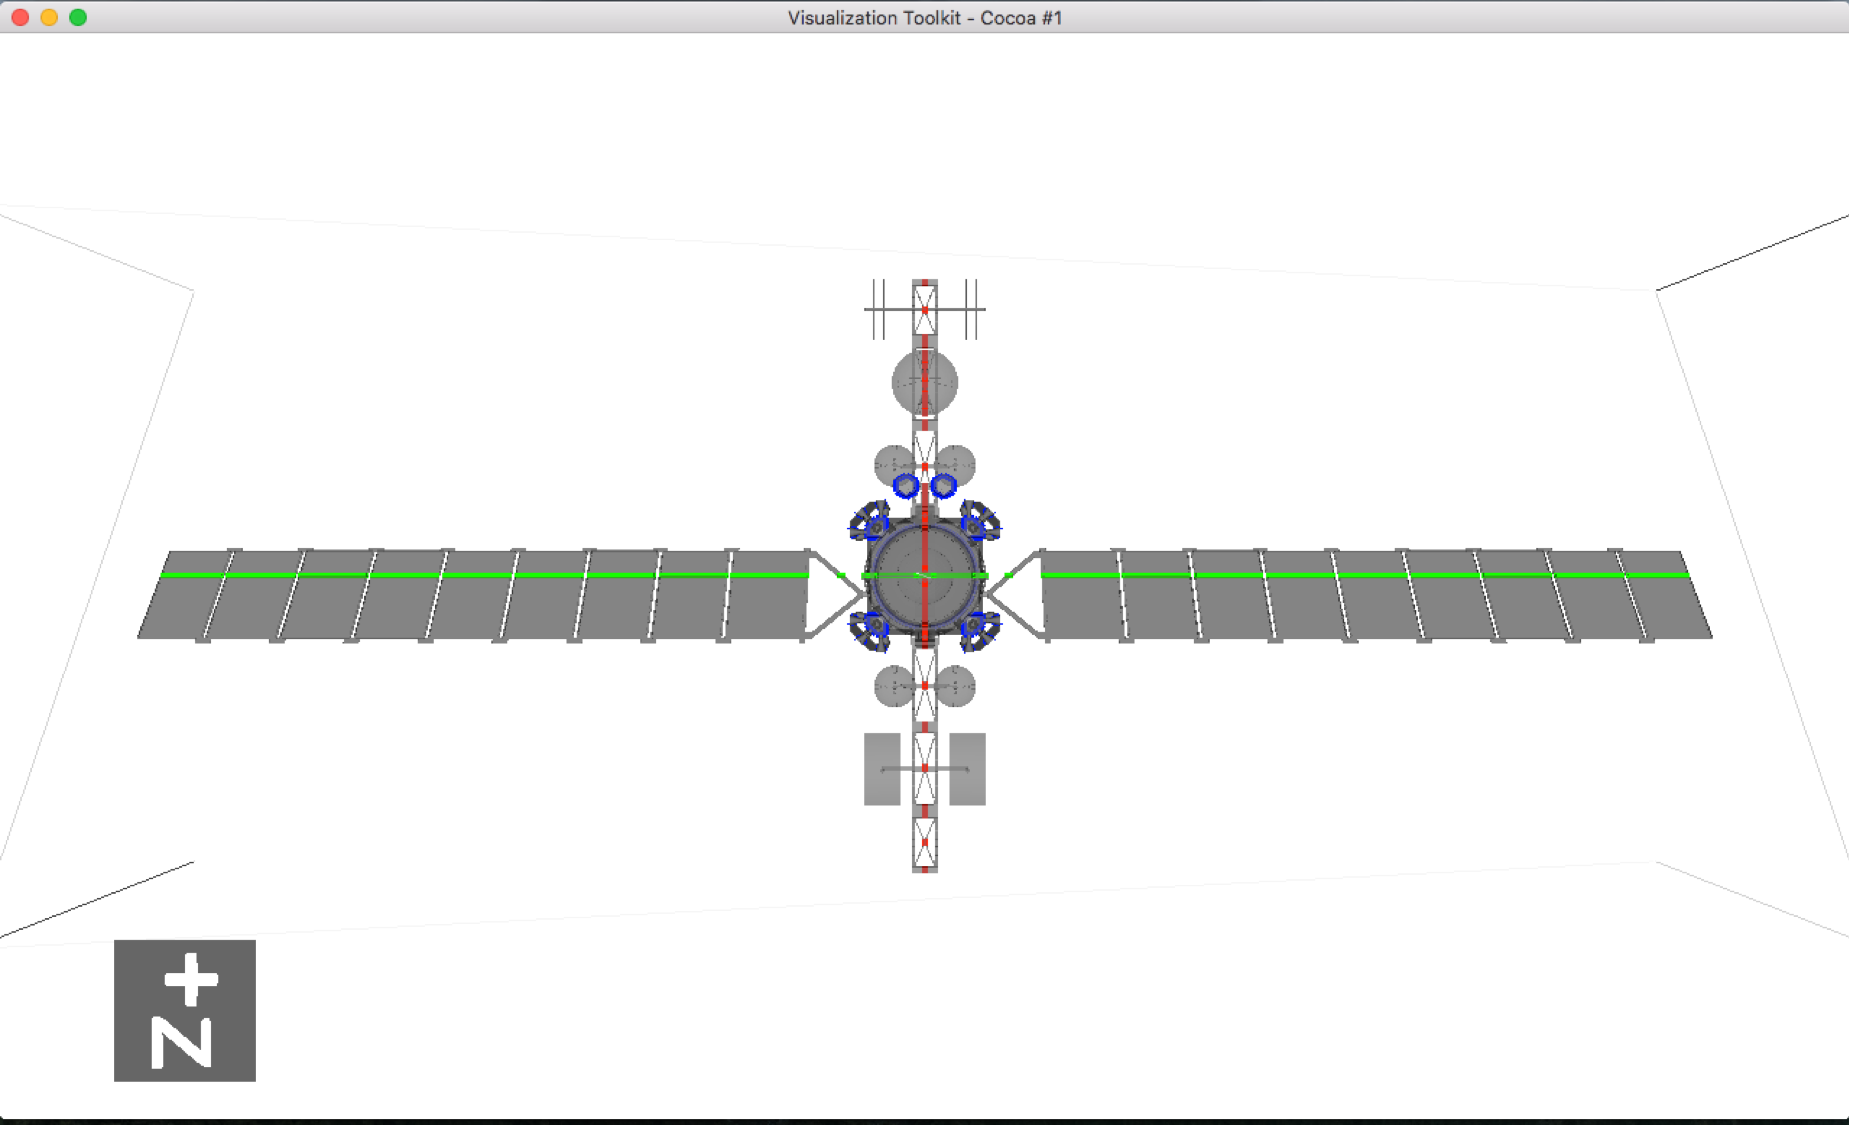
\includegraphics[scale=0.4]{Images//VTK/sat.png}
\caption[width=\columnwidth]{STEP file of a space satellite imported into Pyg4ometry using the Freecad libraries and viewed in VTK.}
\label{sat}
\end{figure}

\begin{figure}[h!]
\centering
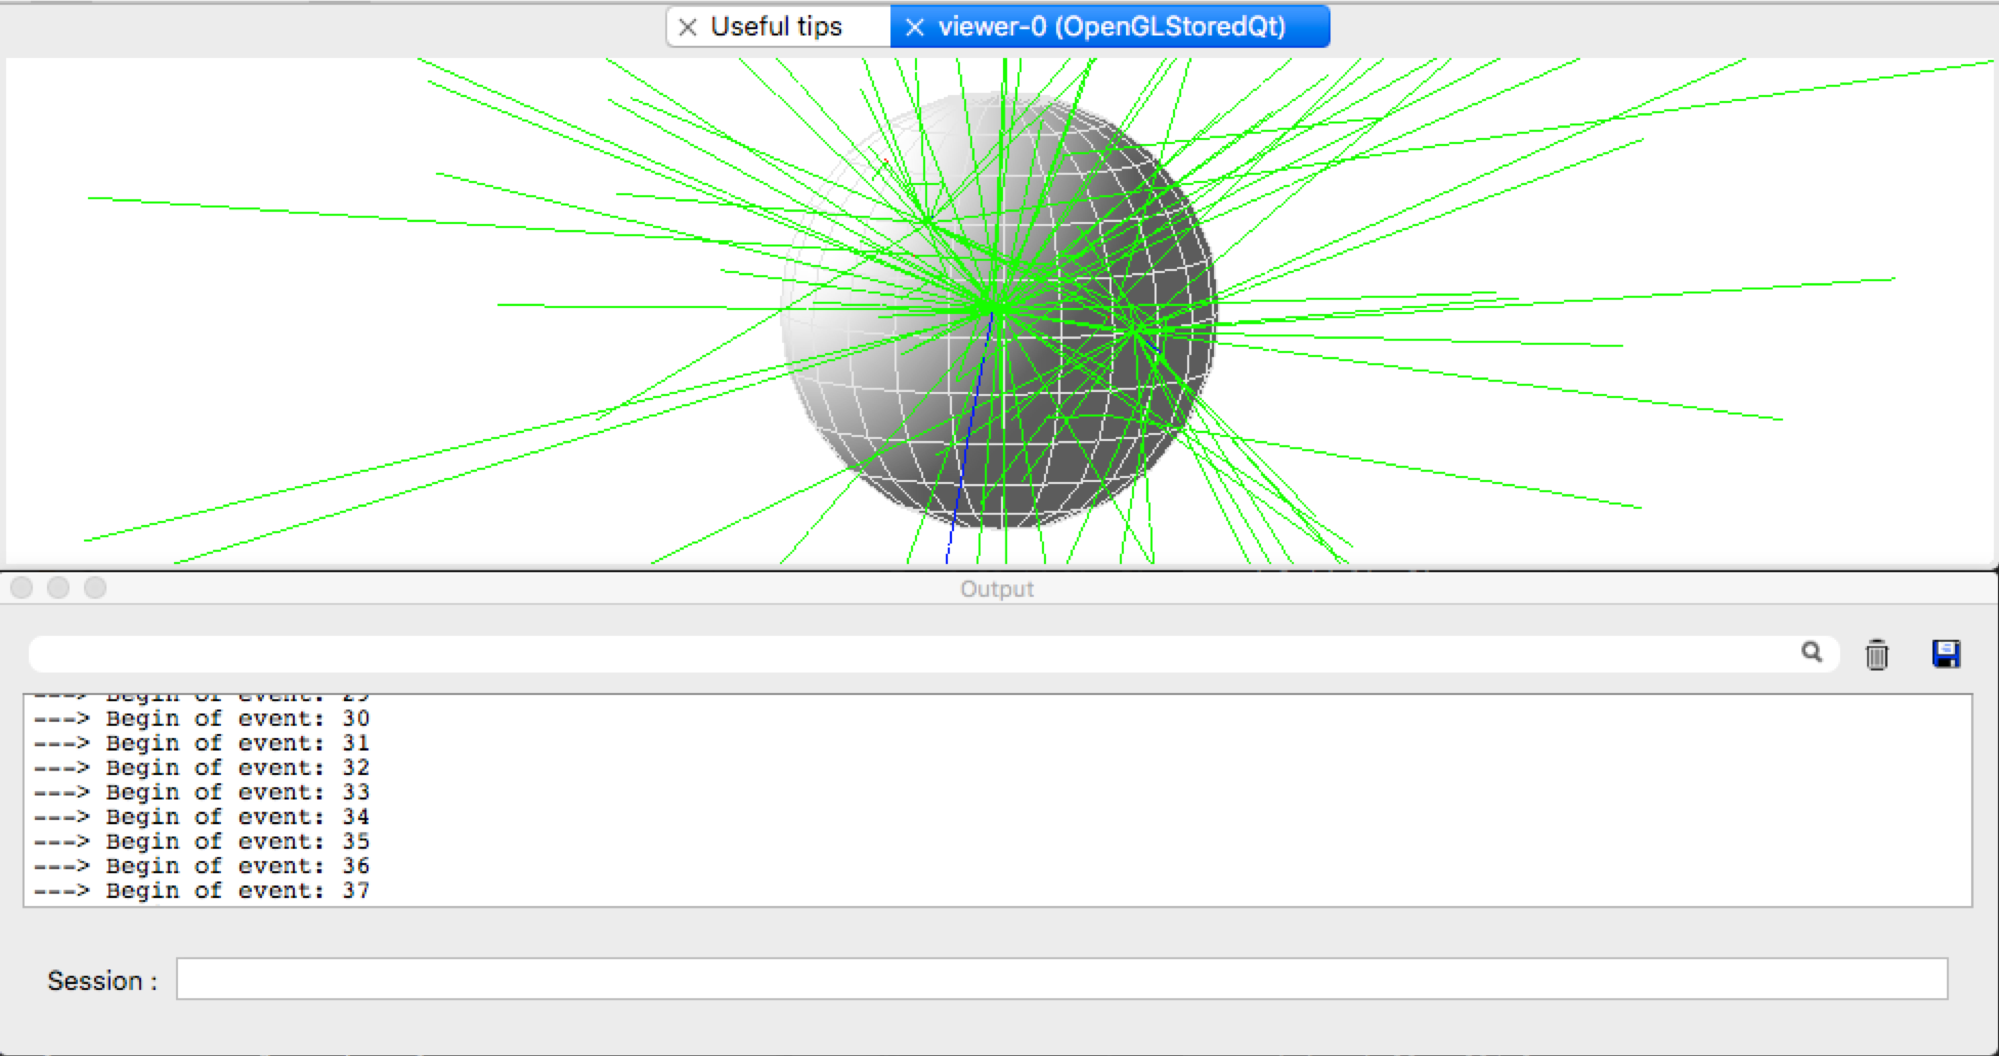
\includegraphics[scale=0.4]{Images//BDSIM//screengrab.png}
\caption[width=\columnwidth]{BDSIM GUI screenshot of particle interaction and output window, using a Geant4 sphere with 10,000 1.3 GeV neutrons.}
\label{screengrab}
\end{figure}


% ------------------------------------------------------------------------------------------------------------------------------
\newpage
\section{Primitive Meshing}
\label{prim}
This section will describe the work done to optimize the Python scripts that generate the three dimensional meshings for the primitive solids within the Pyg4ometry package (Section \ref{pyg}). All the primitive solids used are constructed such that they are compatible with Geant4's solids. It was previously thought that it would be best to use purely triangular based meshes in combination with boolean operations (Section \ref{bool}) to construct the 3D solids. However it had been realised that the computation of triangles and boolean operations in most cases compared with polygons and adapted trigonometry is much more intensive and inefficient. In particular with the curved solids, i.e circular and elliptical based solids, due to the boolean operations generating more complicated meshes. Thus the first part of the major project was to rewrite the meshing scripts for all the curved primitive solids.
\\\\
One of the major improvements to the Pyg4ometry meshing scripts was in the computation of cut up primitive solids. The meshing of hollow or sliced solids were previously constructed by boolean subtractions and intersections, which involves using two or more separate solids and operating on them to create a final single solid. Discussed more in Section \ref{bool}. Which resulted in a very computationally heavy and less aesthetic outcome, where the mesh lines (``slice and stack''), were not meshed in radial directions.

\subsection{Co-ordinate Systems}
\label{cosy}
The various primitive solids are all constructed by using the predefined parameters used by Geant4, to be consistent with Geant4's own solids. The parameters of a 3D solid are properties relating to the co-ordinate system it is constructed in, such as height or radius. The parameters are then used to define the points of the object via basic trigonometry. The order in which the points are appended is also very important and is detailed in Section \ref{order}.
\\\\
The Python meshing scripts for all co-ordinate systems follow a similar structure, of first defining an empty list of faces (polygons). Then running the associated trigonometric equations through a number of loops to generate and append polygons to that list. The number of loops is associated with the number of sections a surface of a solid is being split up into in a given co-ordinate system. The density of the meshing is defined by a user inputted number of slices and stacks, of which the orientations vary with coordinate system. The slice and stack for solids in the cylindrical polar co-ordinate system is demonstrated in Figure \ref{cylmeshin}.

\subsubsection{Cylindrical Co-ordinate System}
\label{cycl}
The meshing for the primitive solids in cylindrical polar co-ordinate systems are constructed by looping through user defined number of slices and stacks (as shown in Figure \ref{cylmeshin}), which the cylinder is being cut into (Listing \ref{code1}). The Loop then creates the co-ordinates for 3 or 4 points at a time using an adaption to the trigonometry in Equations \ref{cyctrig}, which can then be defined as a triangular or polygonal face. The only cases where the new meshing produces triangles is at the top and bottom faces of the cylinder, provided it does not have a minimum radius equal to zero (creating a tube or cone). The same logic for the polygons also applies to triangles, just using 3 vertex points to make a face.

\begin{figure}[h!]
\centering
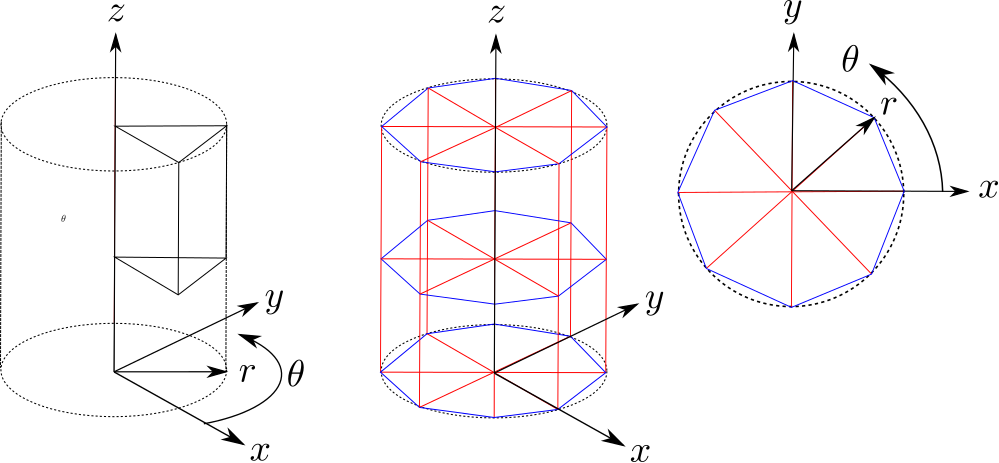
\includegraphics[scale=0.45]{Images//Coords//cyl.png}
\caption[width=\columnwidth]{Diagram showing the meshing method for a cylindrical co-ordinate system, where the red lines indicate the slices (8) and the blue indicate the stacks (2). Diagram drawn using the CAD software Inkscape.}
\label{cylmeshin}
\end{figure}
\vspace{0.3cm}
The trigonometry that converts the points from cylindrical polar co-ordinates to cartesian, are:
\begin{equation}
\begin{aligned}
\label{cyctrig}
& x = r \cos{\theta} \\
& y = r \sin{\theta} \\
& z = z
\end{aligned}
\end{equation}

%\label{code1} 
\newpage
\begin{lstlisting}[language=Python, label=code1, caption=Basic method structure for Pyg4ometry primitive meshing of solids]
polygons = []

for j0 in range(nslice):
    j1 = j0
    j2 = j0 + 1
    
    vertices = []

    for i0 in range(nstack):
          i1 = i0
          i2 = i0 + 1     

\end{lstlisting}
The code in Listing \ref{code1} generates counters so that you can choose from two slices and two stacks, in order to gain the four points surrounding a desired face. These points are then used to define a polygon. 
\\\\
The only time a stack is needed in the cylindrical co-ordinate system is when the solid has a non linear function in the r-z plane. For example a paraboloid (Figure \ref{para}) would need a stack, but a linear cone (Figure \ref{cons}) would not. This is due to the fact how that a plane can not represent a curved surface with a singular face. 

\newpage
\subsubsection{Spherical Co-ordinate System}

The meshing for the primitive solids in spherical co-ordinate systems are constructed by similar means the that of the cylindrical. Just with different trigonometric equations (Equations \ref{trigsph}) as a result of two angle parameters $\phi$ and $\theta$. The stack (blue) and slice (red) for solids in the spherical co-ordinate system works, like the longitude and latitude on a globe, as shown in Figure \ref{sphmeshin}. 
\\\\
The trigonometry that converts the points from spherical co-ordinates to cartesian, are:

\begin{equation}
\begin{aligned}
& x = r \cos{\theta}\sin{\phi}\\
& y = r \sin{\theta}\sin{\phi} \\
& z = z
\end{aligned}
\label{trigsph}
\end{equation}
\begin{figure}[h!]
\centering
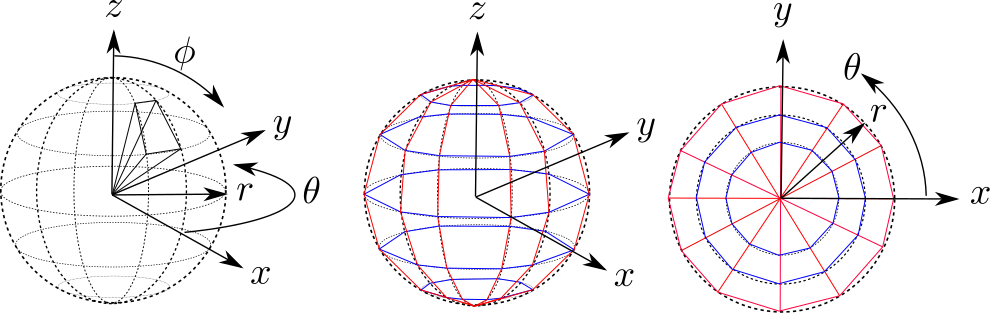
\includegraphics[scale=0.5]{Images//Coords//sph.png}
\caption[width=\columnwidth]{Diagram showing the meshing method for a spherical co-ordinate system\\
Red = Slices (12)\\
Blue = Stacks (6)\\
 Diagram drawn using the CAD software Inkscape.}
\label{sphmeshin}
\end{figure}

\noindent The structure of the code for a spherical system is the same as used in Listing \ref{code1}.\\\\
\noindent The only time triangles are constructed in the spherical co-ordinate system is if the solid has a complete pole at the top or bottom of the solid. The solids constructed in the spherical always have both a stack and a slice.

%\begin{lstlisting}[language=Python, caption=Python example]
%for j0 in range(nslice):
%    j1 = j0
%    j2 = j0 + 1
%
%    for i0 in range(nstack):
%          i1 = i0
%          i2 = i0 + 1
%\end{lstlisting}

\newpage
\subsubsection{Toroidal Co-ordinate System}

The toroidal co-ordinate system is a special case and is only needed, for toroidal based solids. A toroidal shape is much harder to visualise a stack and slice, due to the fact it is a rotating co-ordinate system. A toroidal slice is an $R_{Torus}$ radial cut taken out of the angle $\phi$, as shown in Figure \ref{tormeshin}. The toroidal stack is a $R$ radial cut out of the angle $\theta$. 
\\\\
The trigonometry that converts the points from toroidal co-ordinates to cartesian, are:

\begin{equation}
\begin{aligned}
& x = R_{Torus} + R\cos{\theta}\cos{\phi} \\
& y = R_{Torus} + R\cos{\theta}\sin{\phi} \\
& z =  R\sin{\theta} 
\end{aligned}
\end{equation}

\begin{figure}[h!]
\centering
\includegraphics[scale=0.35]{Images//Coords/torus_coords.png}
\caption[width=\columnwidth]{Diagram showing the meshing method for a toroidal co-ordinate system. Diagram drawn using the CAD software Inkscape.}
\label{tormeshin}
\end{figure}

\subsection{Plane Direction}
\label{order}
One key thing to be taken into account is the convention being used in the code for the order in which points are appended to make a plane, i.e to define a face on a solid. This is important as the direction the normal of the plane points in, dictates wether a face is considered an inside or outside face on the given solid. Getting this order incorrect, will lead to missing faces, when the meshing is made. The concept is demonstrated in Figure \ref{pointsorder}.

\begin{figure}[h!]
\centering
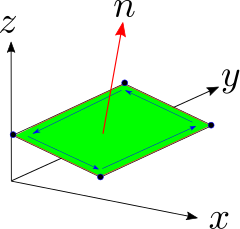
\includegraphics[scale=0.75]{Images//append_points//Point_Appending_Order.png}
\caption[width=\columnwidth]{Diagram showing the order convention of appending points to define the normal to a plane. Diagram drawn using the CAD software Inkscape.}
\label{pointsorder}
\end{figure}
\noindent The simplest way to test this is by performing boolean operations with a box, as the boolean operation will only work nicely if all the planes are correct on both shapes. This test only works for the visualiser in BDSIM as it uses Geant4, which displays face directions. VTK inside Pyg4ometry is much more lenient and will display solids even if their normals are incorrect, giving you a false idea of what is being displayed.

\subsection{New Meshing of Curved Primitive Solids}
In total there are 12 curved primitive solids, of which many of the examples and concepts are very similar. Therefore only a few select solids will be discussed in this section, but the remaining solids and their development can all be viewed in Appendix \ref{app1}. The naming convention of the solids being in this project and within this report are the ones used by Geant4.
\\\\
One of the curved solids is the polycone, the old and new meshing development of the polycone is shown in Figure \ref{polypic1}. It can be seen that in this example that the meshing at the top and bottom faces becomes more radially uniform. This is due to the replacement of boolean subtractions with simple trigonometry within the new meshing algorithm for the polycone.

\begin{figure}[h!]
\centering
\begin{minipage}{.4\textwidth}
  \centering
  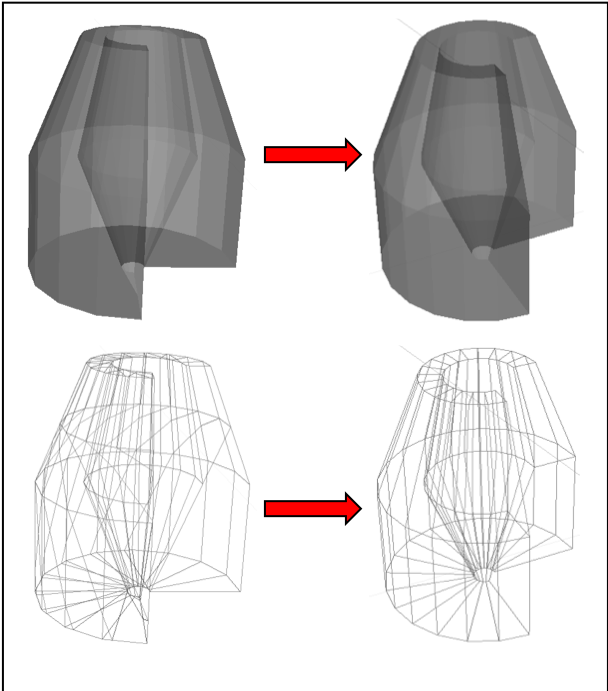
\includegraphics[height=1\linewidth]{Images//Meshes//polycone.png}
  \captionof{figure}{Meshing Development \\for polycone (Solid \& Mesh View)}
  \label{polypic1}
\end{minipage}%
\begin{minipage}{.4\textwidth}
  \centering
  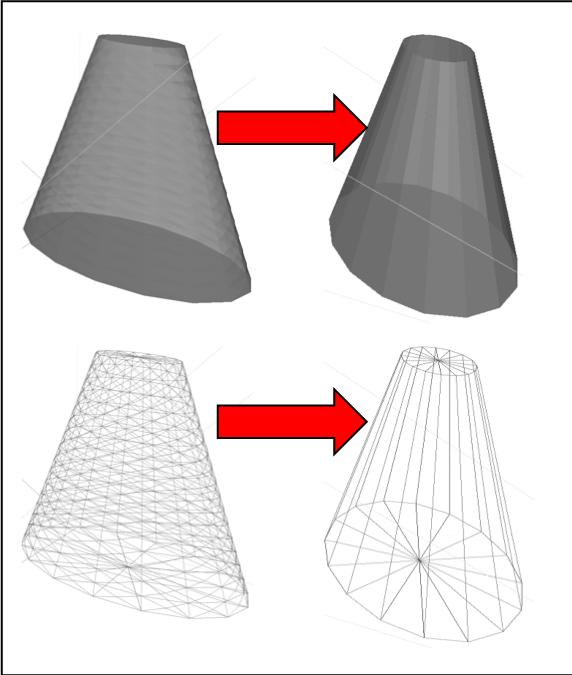
\includegraphics[height=1\linewidth]{Images//Meshes//ellipticalcone.png}
  \captionof{figure}{Meshing Development \\for ellipticalcone (Solid \& Mesh View)}
  \label{elco1}
\end{minipage}%
\end{figure}

\noindent Another curved solid that was remeshed is the ellipticalcone, as seen in Figure \ref{elco1}. Despite having no boolean operation to generate this solid, the meshing is still improved by replacing all the unessessary triangular faces with quadrilateral ones. The stack was also removed as for the cone the faces in the r-z plane (in cylindrical co-ordinates) is a linear function.

\subsubsection{Degenerate Points}
Multiple meshing points occupying the same area can spring a few errors, sometimes without entirely crashing the code, making it a hard error to identify. It is typically given away when a $DivisionByZero$ error occours, within the pycsg meshing of a solid. You can identify wether this is the error by debugging each polygon and triangle in a mesh, looking out for a face that has two or more vertices with the same $(x,y,z)$ coordinates. This typically happens when you mean to mesh a triangle, but are still using the format for meshing a quadrilateral face. Or it can be due to the incorrect choice of an incorrect stack and slice iteration when constructing a face, as mentioned before in Section \ref{cosy}.

\subsubsection{Boolean Operations}
\label{bool}
One of the largest improvements to the performance of the new meshing methods compared with the previous methods, is the discarding of boolean operations in order to create hollow or cut-up primitive solids. The idea can be clearly seen in Figure \ref{booly}, where you conduct basic operations on simple solids, resulting in a complex solid being made.
\\
\begin{figure}[h!]
\centering
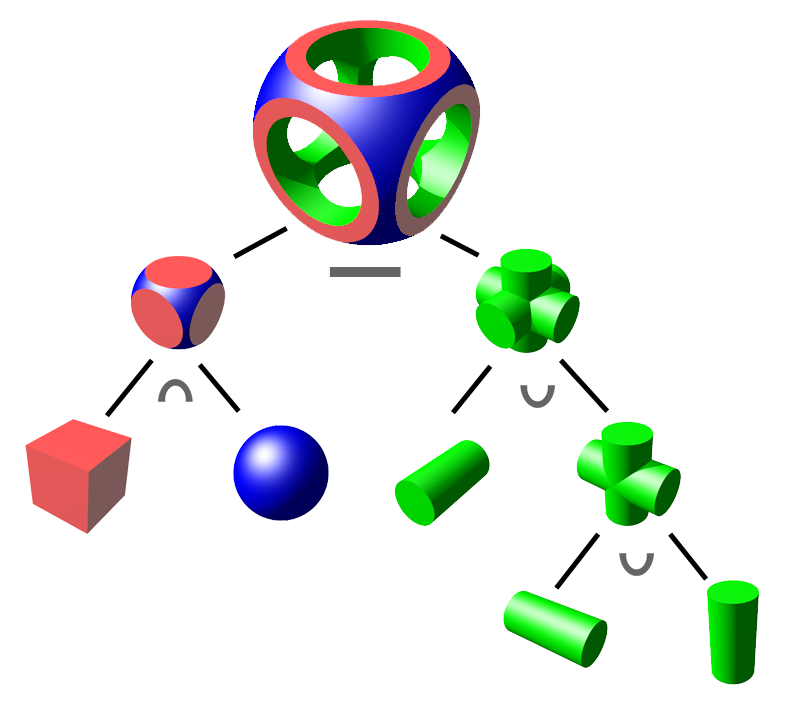
\includegraphics[scale=0.3]{Images//Booleans//Boolean.png}
\caption[width=\columnwidth]{A diagram showing the basic method of constructing a more complicated 3D solid out of boolean operations with simpler primitive solids.\\
- = Boolean Subtraction\\
n = Boolean Intersection\\
u = Boolean Unions}
\label{booly}
\end{figure}

\noindent The Figures \ref{uni} \& \ref{sub} are of the meshed boolean union and subtraction of a box with a hollow sphere (in solid view). The coloured lines are representing the perpendicular planes in which the final object is placed in. These were made in the process of checking the normals before passing them into BDSIM to undergo interactions.
\\
\begin{figure}[h!]
\centering
\begin{minipage}{.4\textwidth}
  \centering
  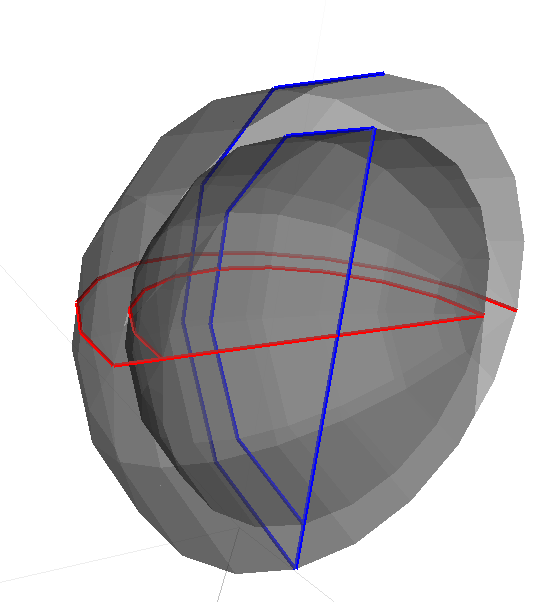
\includegraphics[height=0.5\linewidth]{Images//Booleans/SphereUnion.png}
  \captionof{figure}{Example screenshot of\\ a Boolean Union produced in\\ Pyg4ometry \& viewed in VTK.}
  \label{uni}
\end{minipage}%
\begin{minipage}{.4\textwidth}
  \centering
  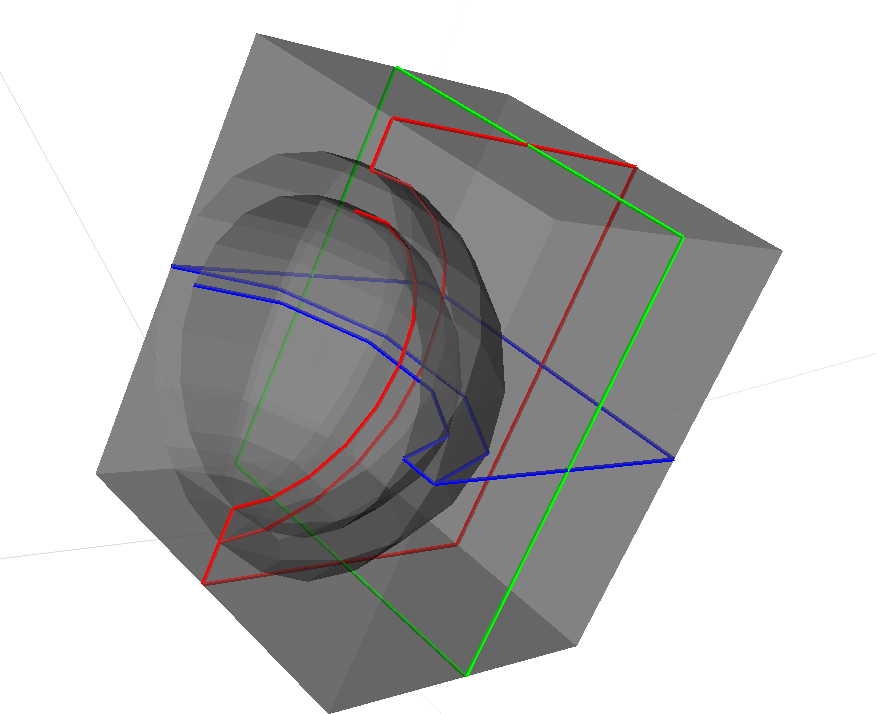
\includegraphics[height=0.5\linewidth]{Images//Booleans//SphereSubtraction.png}
  \captionof{figure}{Example screenshot of \\ a Boolean Subtraction produced\\ in Pyg4ometry \& viewed in VTK.}
  \label{sub}
\end{minipage}%
\end{figure}



\noindent The old meshing algorithms would heavily rely on these operations. The old meshing algorithms used intersections to slice solids, as seen in Figure \ref{ctub}, and subtractions to make solids hollow of cut-up, as seen in Figure \ref{Sphere}. For example Tubs is made from two cylinders being subtracted in order to create a tube as seen in Figure \ref{tubspic}. The boolean operations worked, however are very computationally heavy compared with that of the adapted trigonometry applied in the new method. This is the case especially when one or more of the orginal solids is curved in structure. Another thing the boolean operations affected was the appearance of the mesh its self, the boolean operations worked by trying to identify common mesh points then remesh. This created a lot of non radially uniform mesh sections as seen in solids such as the polycone and Tubs , which do not appear in the new meshing algorithms.\\



\newpage
\subsection{Meshing Performance Testing}
\subsubsection{Polygon Count}
One way in which the meshing performance of the Pyg4ometry primitive solids is tested, is by counting the number of polygons produced by both the old and new meshing alogrithms. I.e counting the number of triangular and quadrangular faces on a solid, in order to make a comparison. A plot for each primitive solid counting its number of generated polygons was produced.
\\\\
They were generated by varying the user inputted number of slices across a range. Most were put through the range of (10-100) slices, whilst keeping the number of stacks at a constant 10. However a few old solid meshings took too long to produce at higher mesh densities. Leading to a few solids only being measured across a shorter range of slices e.g the old Hyperboloid meshing was left to run for over a couple hours and only collected data up to a slice of 50.  \\

\begin{figure}[h!]
\centering
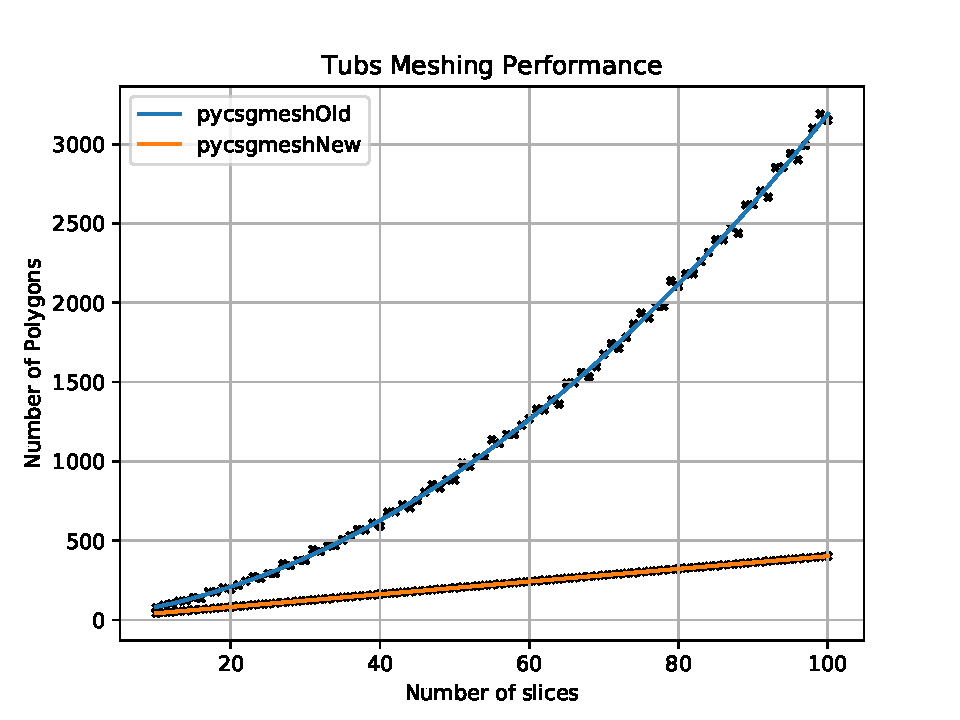
\includegraphics[scale=0.6]{Images//Quad_fits//Tubs_quad.pdf}
\caption[width=\columnwidth]{A plot showing the comparison of the number of polygons (and triangles) generated by the new and old meshing methods, across a range of slices 10-100.}
\label{conts}
\end{figure}

\noindent Figure \ref{conts} is one of many plots, which are all displayed in the Appendix \ref{app1}. As you can see in Figure \ref{conts} the new meshing function is much more computationally reduced compared with the old meshing function. The number of polygons increases more uniformly and linearly for the new pycsgmesh function. The old function exhibits a more scatters and quadratic relationship. This can be seen by the values tabled in the Appendix, which contains the quadratic fitting parameters to all these plots. If you extrapolated both graphs it is clear than the new mesh is not only improving the structural appearance of the meshed solids, but also saving large amounts of computational power and time.
\\\\
\noindent The polygon count plots for the remaining primitive solids can be found in the Appendix \ref{app1} and a table of parameters for the quadratic fits can also be found in the Appendix \ref{tab1}. 

\newpage
\section{BDSIM Interactions}
\label{int}
The second aim of this project was to measure how the physics is altered, between the new and old meshings as the mesh density is varied. As mentioned before Geant4 already has its own set of primitive solids, which can be used as a guideline for comparison, due to no slice and stack dependence. The physics being measured will be features such as the trajectories and energy deposition, through solids.

\begin{figure}[h!]
\centering
\includegraphics[scale=0.33]{Images//BDSIM//titanium.pdf}
\caption[width=\columnwidth]{Titanium Sphere generated with new meshing interacting with 1.3 GeV electrons in BDSIM.}
\label{black}
\end{figure}

\noindent Within BDSIM the charge of a particle is represented by its colour, green = neutral, blue = positive and red = negative, as seen in Figure \ref{black}, where electrons and secondaries are being radiated from the centre of a meshed sphere. A secondary particle is anything that is produced as a result of the initial particles interacting with the solid, therefore a secondary itself can produce anther particle which is considered to also be  a secondary particle. The probability of certain events and the scattering of a particles trajectories is generated by a Monte Carlo simulation. Each seed that produces a different outcome in the Monte Carlo simulations has a unique seed number. This allows a particular event to be repeated with the same physics, which is key to this project when it comes to comparing the interactions of two different objects under the same conditions. The other properties of the particle and physics processes that may occur can also be user defined to tweak the experiment. Properties such as the particles initial energy, wether secondaries get produced and much more. The seeds used in this project could not be logically chosen due to the fact they are generated via the Monte Carlo simulation. Therefore they were selected by running a lot of test runs in BDSIM to see which seeds generate a decent amount of secondaries.
\\\\
BDSIM works by running a GMAD file and then outputs  a ROOT (Section \ref{root}) file with the option of using the GUI, allows the user to visualise the interactions in an interactive 3D environment. A GMAD file contains the basic information needed to produce an interaction in BDSIM, i.e a particle and path to file of the target object (Typically of the format GDML). The option ``physicsList'' defines the physics which is used for the interaction, for the project the option was set to``g4FTFP\_BERT'', which contains all the standard electomagnetism and particle physics required for this project. The ROOT file contains a detailed analysis of the interaction. One of the elements analysed within this project is the CPU duration time distribution of an interaction in BDSIM.
\\\\
The shape chosen to be tested within BDSIM for this project was the sphere, which is made of a minimum and maximum radius, making it a hollow solid. The reason a sphere was chosen because it is the ideal shape testing radiation in all directions, as its thickness can be controlled radially. As seen in Figure \ref{sphbd} the sphere was orginally chosen to be orientented such that the particle beam is fired from the centre of the sphere outwards. The conversion from a Pyg4ometry mesh into a Geant4 tessellated solid, results in only triangular faces. This is why all the quadrilateral faces are cut into two in Figure \ref{sphbd}.

\begin{figure}[h!]
\centering
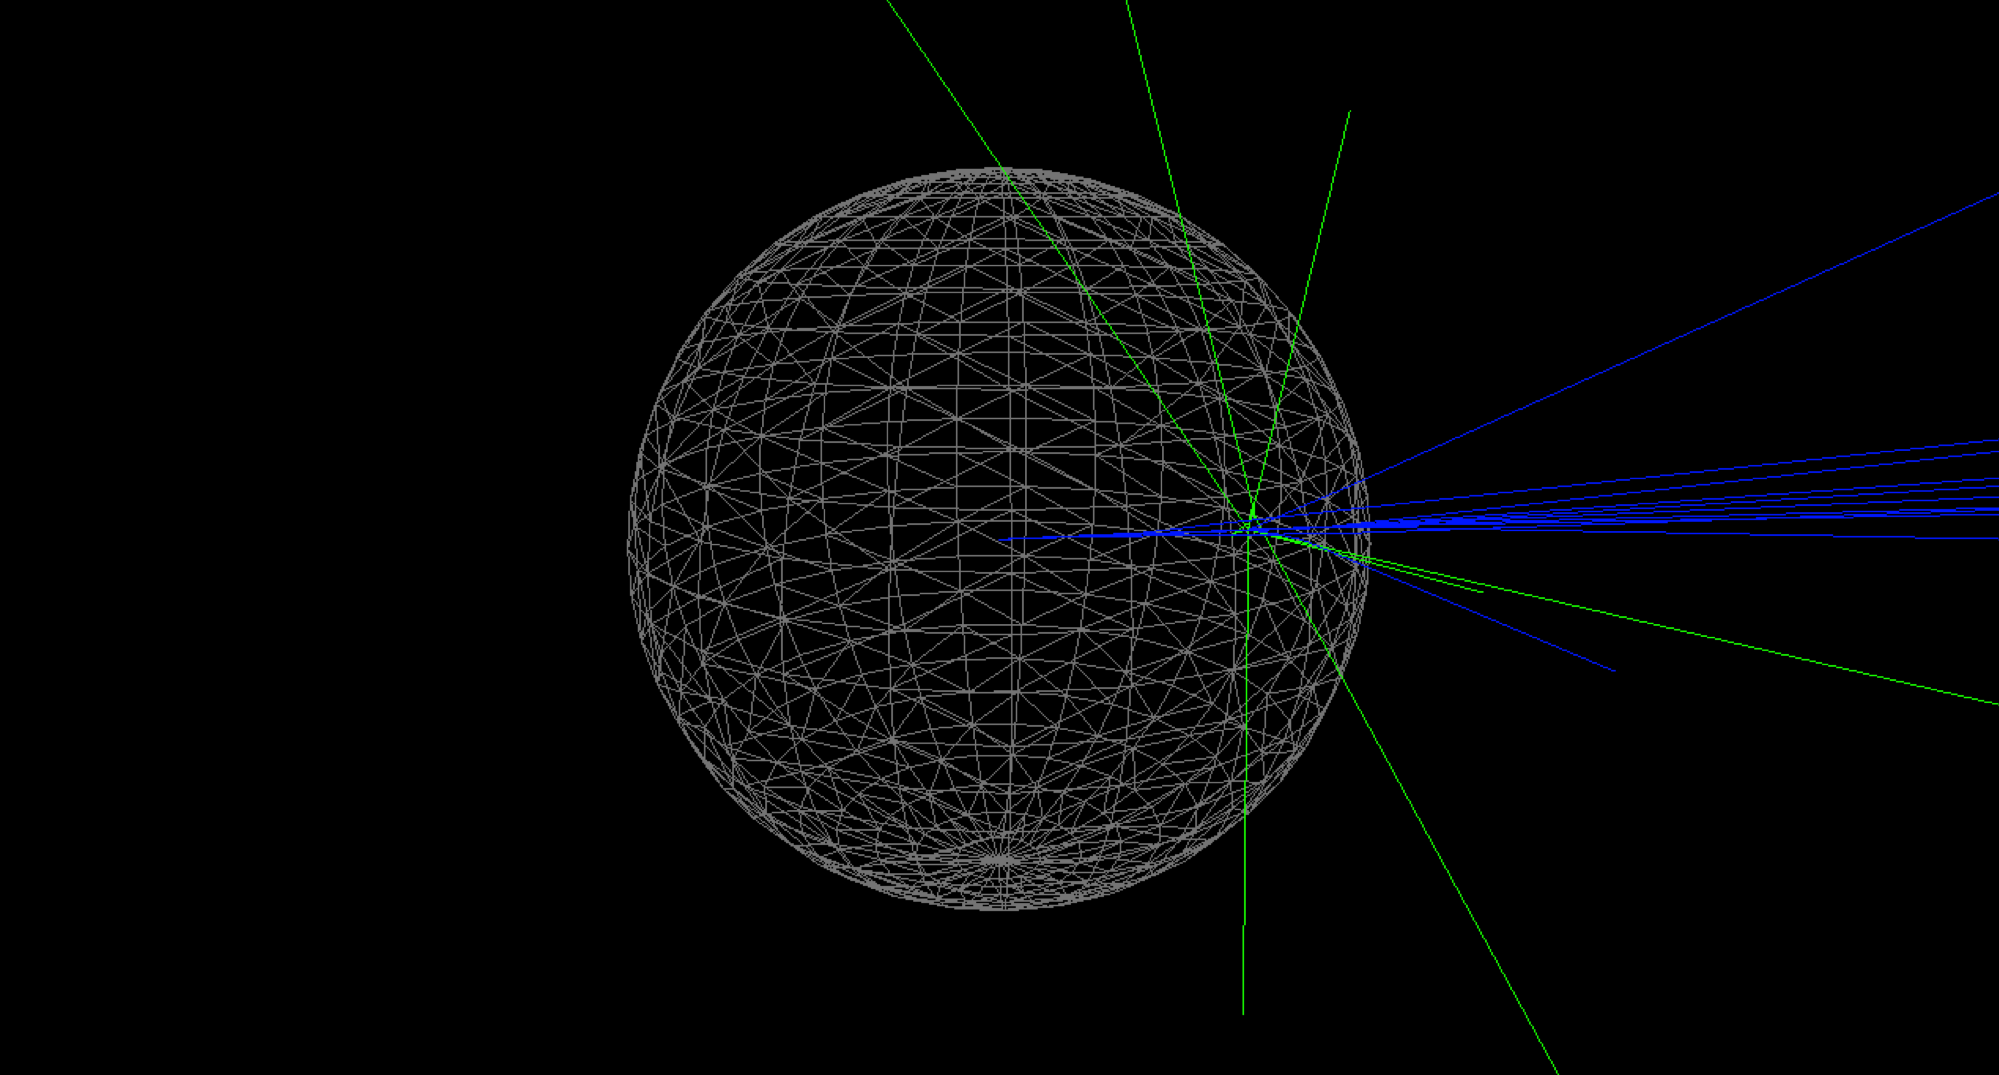
\includegraphics[scale=0.35]{Images//BDSIM//ProtonSphere2.png}
\caption[width=\columnwidth]{BDSIM screenshot of 10 1.3 GeV protons interacting with a Iron sphere, which has been constructed using the new meshing scripts. Mesh reseloution is a stack \& slice of 25 \& 25. (Shown in mesh view)}
\label{sphbd}
\end{figure}

\noindent One way that was though to analyse the energy deposition of the interactions, was to look at the CPU duration times as the mesh densities are increased. In this scenario the Geant4 solid was used as a guideline as it does not depend on a user defined stack \& slice. 

\subsection{Iron Sphere Interactions}
rmin = 8mm\\
rmax = 10mm\\
1.3Gev protons\\
10,000\\

\begin{figure}[h!]
\centering
\begin{minipage}{.5\textwidth}
  \centering
  \includegraphics[height=0.75\linewidth]{Images//CPU//Total_plot.pdf}
  \captionof{figure}{A plot showing mean\\ CPU duration of 10,000 protons\\ interacting with a Iron sphere of\\ various meshed forms.\\}
  \label{cons}
\end{minipage}%
\begin{minipage}{.5\textwidth}
  \centering
  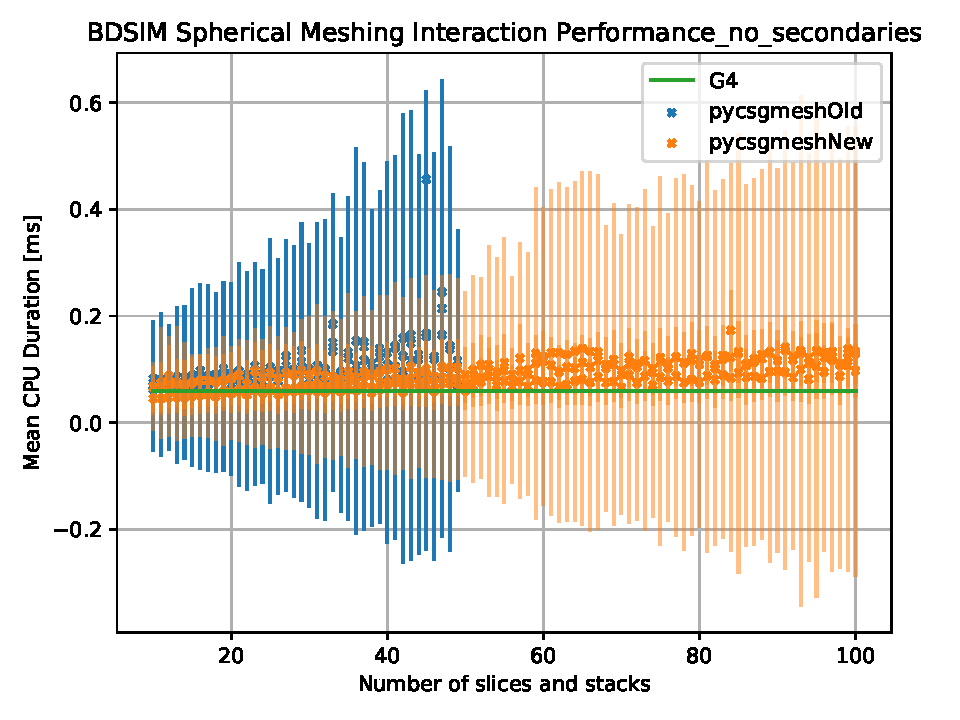
\includegraphics[height=0.75\linewidth]{Images//CPU//Total_Plot_no_secondaries.pdf}
  \captionof{figure}{ A plot showing mean\\ CPU duration of 10,000 protons\\ interacting with a Iron sphere of\\ various meshed forms, with\\ secondary particles disabled.}
  \label{fig:test2}
\end{minipage}%
\end{figure}

\begin{figure}[h!]
\centering
\begin{minipage}{.5\textwidth}
  \centering
  \includegraphics[height=0.75\linewidth]{Images//CPU//Total_plot_with_offset.pdf}
  \captionof{figure}{A plot showing mean\\ CPU duration of 10,000 protons\\ interacting with a Iron sphere of\\ various meshed forms, with\\ an 20 mm of set in the Z-axis.}
  \label{cons}
\end{minipage}%
\begin{minipage}{.5\textwidth}
  \centering
  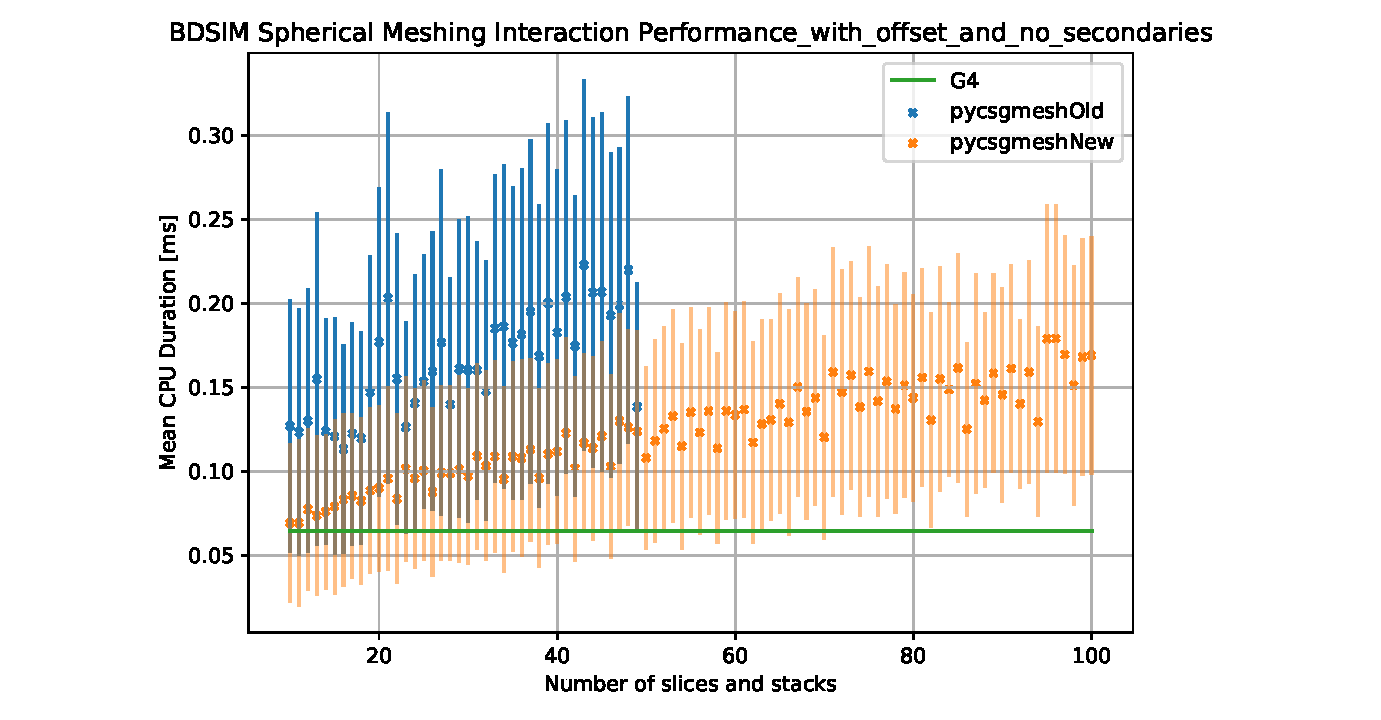
\includegraphics[height=0.75\linewidth]{Images//CPU//Total_Plot_with_offset_and_no_secondaries.pdf}
  \captionof{figure}{ A plot showing mean\\ CPU duration of 10,000 protons\\ interacting with a Iron sphere of\\ various meshed forms, with\\ secondary particles disabled, with\\ an 20 mm of set in the Z-axis and secondaries disabled.}
  \label{fig:test2}
\end{minipage}%
\end{figure}

\noindent From FIgures \ref{} and \ref{}, you can see that as the number of stack and slice is increased the mean CPU duration for the protons increases at a slower rate for the new meshing. The old meshing would only meshed up to a maximum reseloution of slice = 48 and stack =48, before it would max out pythons recursion limit. Where as the new meshing could go to 100 stack, 100 slice with out any issues at all.
\\\
\noindent It was orginaly thought that the standard deviations of the CPU durations was related to the number of secondaries being produced. However this was disproved by Figure \ref{}, where the same test was conducted with the BDSIM option that disables secondary particles from being produced implemented.

\subsubsection{Error Reduction}
To reduce the standard deviation of a data set the number of events needs to be increased, this proved by the relation ship shown in Equations \ref{std}. The relationship between the standard deviation and number of events is inversely square root proportional. Therefore the standard deviation should decrease with a increasing N.

\begin{equation}
\begin{aligned}
& \bar{x} = \frac{1}{N}\sum{x_i}\\
& \sigma = \sqrt{\bar{x}^2} = \sqrt{\frac{1}{N}\sum{(x_i - \bar{x}})^2}\\
& \sigma \propto \frac{1}{\sqrt{N}} 
\end{aligned}
\label{std}
\end{equation}

However Figure \ref{} shows...\\
\begin{figure}[h!]
\centering
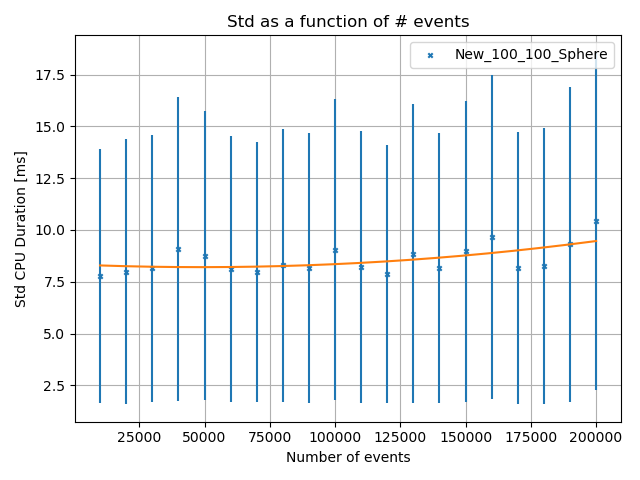
\includegraphics[scale=0.5]{Images//Error//std_N.png}
\caption[width=\columnwidth]{BDSIM screenshot of 200 1.3 Gev protons interacting with a Iron sphere, generated with the new meshing using a stack \& slice of 10 \& 10. (Shown in mesh view)}
\label{sphbd}
\end{figure}

The error bars are still very big so it was proposed to use the standard error of the main as an alternative. As well as as investigation for varying energy and the material of the target.

\subsection{Choice of Materials}
When creating meshed solids, you have the choice of material. Figure \ref{novar} shows the CPU duration time distributions for electrons interactions with Geant4 spheres constructed of different Geant4 materials across a range of energies in BDSIM. The energy range is relatively low (25 MeV $\rightarrow$ 100 MeV), this is due to the run time of the interactions increasing with energy. The run time is heavily linked to the number of secondary particles which is a function of energy. This is proven by the fact that it can be seen that as the energy is increased the width of the distribution increases. This widening is due to the number of secondary particles being produced, the more energetic an interaction the further the particle will penetrate a solid and ionise along the way generating more secondaries.

\begin{figure}[h!]
\centering
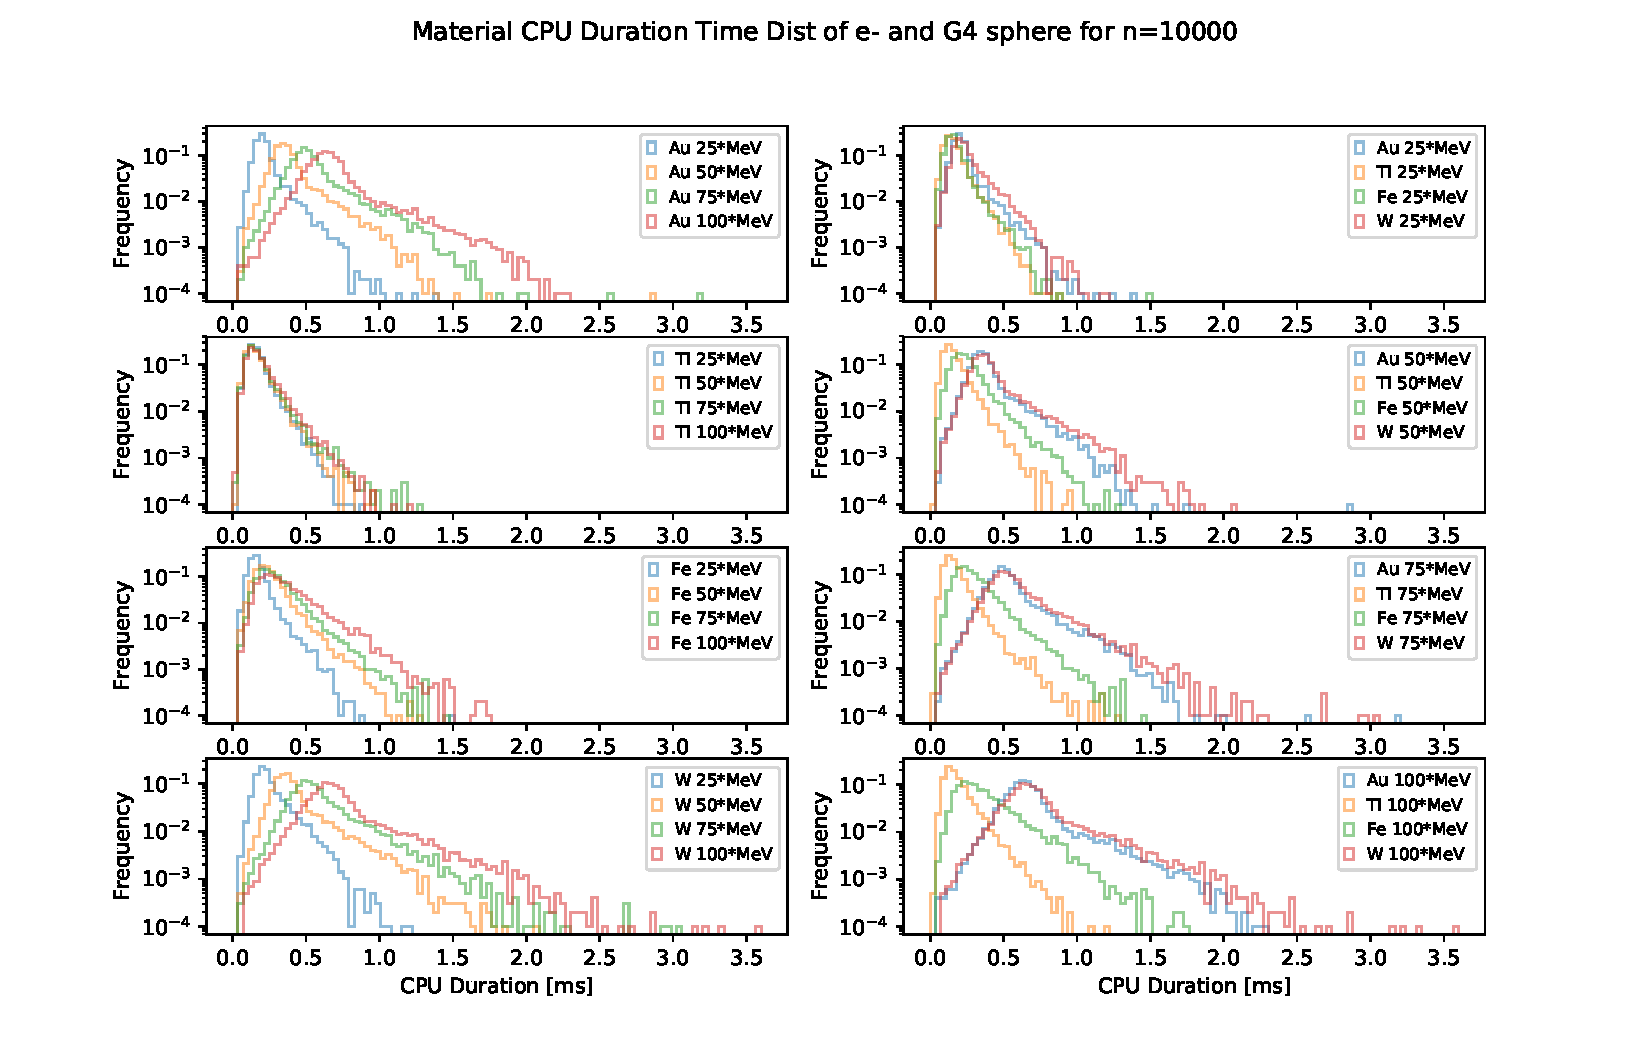
\includegraphics[scale=0.6]{Images//Materials//not_Varied_by_radius_and_secondaries.pdf}
\caption[width=\columnwidth]{Histograms showing the CPU duration distributions of varying Geant4 materials and particle energies in BDSIM on a Geant4 sphere. The left 4 histograms show the distributions show the varying of energy apon each material. The right 4 histograms show the varying of material at each set energy. Each plot is normalised by the initial 10,000 electrons in each event.}
\label{novar}
\end{figure}

\noindent The dimensions of the spheres used in Figure \ref{novar} were set to a minimum radius of 1 micron and a maximum radius of 20 mm. It was then proposed that the radius of thickness could be scaled with respect to the stopping distance of the material it is travelling through, in order to eliminate material as a variable. The radius of thickness $\Delta R$ can be seen depicted in Figure \ref{deltar}, where $\Delta R = R_{Max} - R_{Min}$. The next Section discusses the stopping power of materials in more detail.

\begin{figure}[h!]
\centering
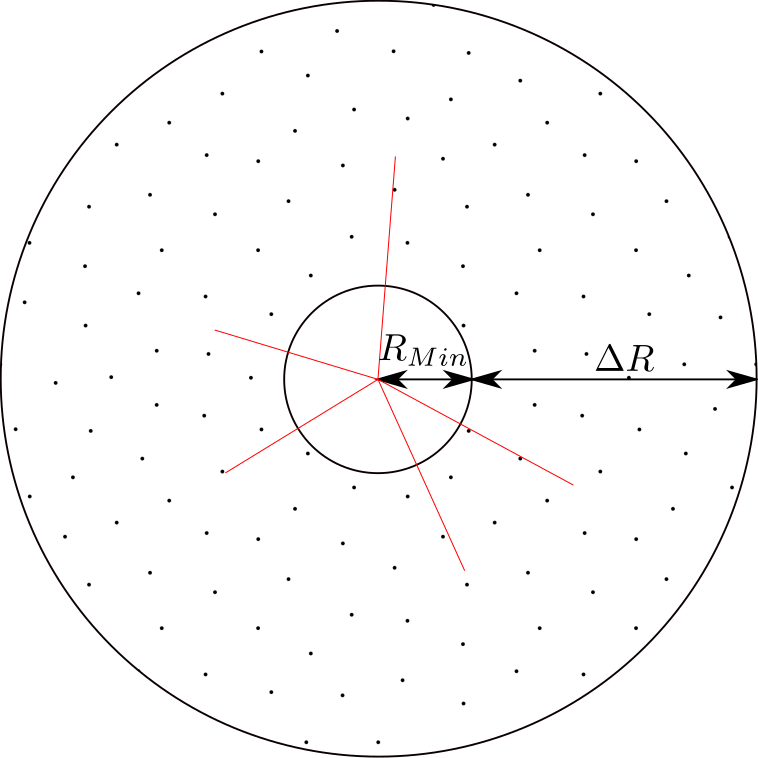
\includegraphics[scale=0.2]{Images//Materials//RMAX.png}
\caption[width=\columnwidth]{A diagram depicting a crossection of a sphere, which has a minimum and maximum radius. The diagram was drawn using the CAD software Inkscape.}
\label{deltar}
\end{figure}


\newpage
\subsubsection{Stopping Power}
\label{stop}
Stopping power is the force that acts against the motion of a particle within in a material, causing it to lose energy. The Geant4 example ``TestEm0'' outputs the stopping power and distances for a given material and particle energy. If the energy of the incident particle and the stopping power of the material is known, a stopping distance can be calculated. The values for stopping power in this project are calculated by the TestEmo example, which extracting values from a Geant4 data lists and then interpolates or extrapolates between them, as the stopping power is a function of. The extracted stopping powers match with values found in other studies, such as \cite{stpdat}.
\\\\
Figure \ref{tung} shows a sphere made of G4\_W, undergoing interactions with 100 different energy electrons. The spheres radius of thickness is set to the be the stopping distance for G4\_W interacting with a 1 TeV electron. It can be seen that when the energy of the electrons is 1 GeV, which is below the 1 TeV (the stopping distance energy for this situation), the tracks of the interactions are al contained within the sphere. The opposite happens when the electrons energies are more than 1TeV, where most if not all of the particle tracks leave the sphere. 

\begin{figure}[h!]
\hspace*{1.4cm}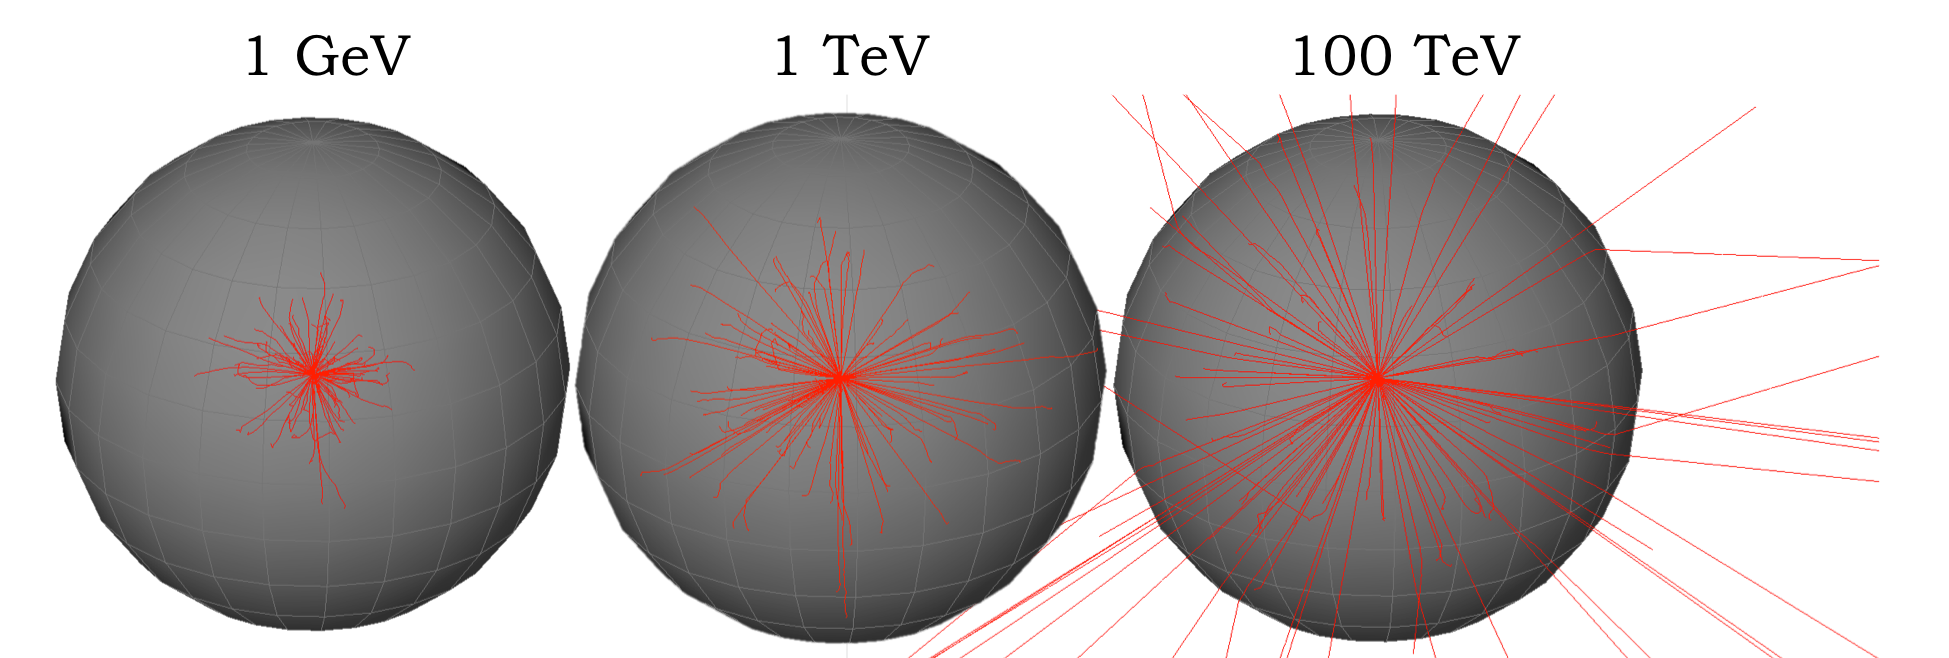
\includegraphics[scale=0.5]{Images//BDSIM//Tungsten_Sphere.png}
\caption[width=\columnwidth]{Screenshots of 1 GeV, 1TeV \& 100 TeV electrons interacting with a tungsten sphere. Where the radius of thickness is set to the extracted Geant4 stopping distance of a 1 TeV electron in tungsten.}
\label{tung}
\end{figure}

\noindent With the stopping power in mind Figure \ref{novar} was reproduced, but instead of using the same dimensions for each sphere, $\Delta R$ was scaled by the stopping distance. The radius of thickness is set to be the extracted stopping distance for a 100 MeV electron interacting with the material in question. The values of $\Delta R$ are shown in Table \ref{rs}.

\newpage
\begin{table}[h!]
\centering
\begin{tabular}{|l|l|}
\hline
Material & $\Delta R$ [mm] \\ \hline
G4\_Au &  9.89382\\ \hline
G4\_Ti &  33.6854\\ \hline
G4\_Fe &  62.3434\\ \hline
G4\_W &  10.1631\\ \hline
\end{tabular}
\caption{A table showing the values of $\Delta R$ used in Figure \ref{var}.}
\label{rs}
\end{table}

\begin{figure}[h!]
\centering
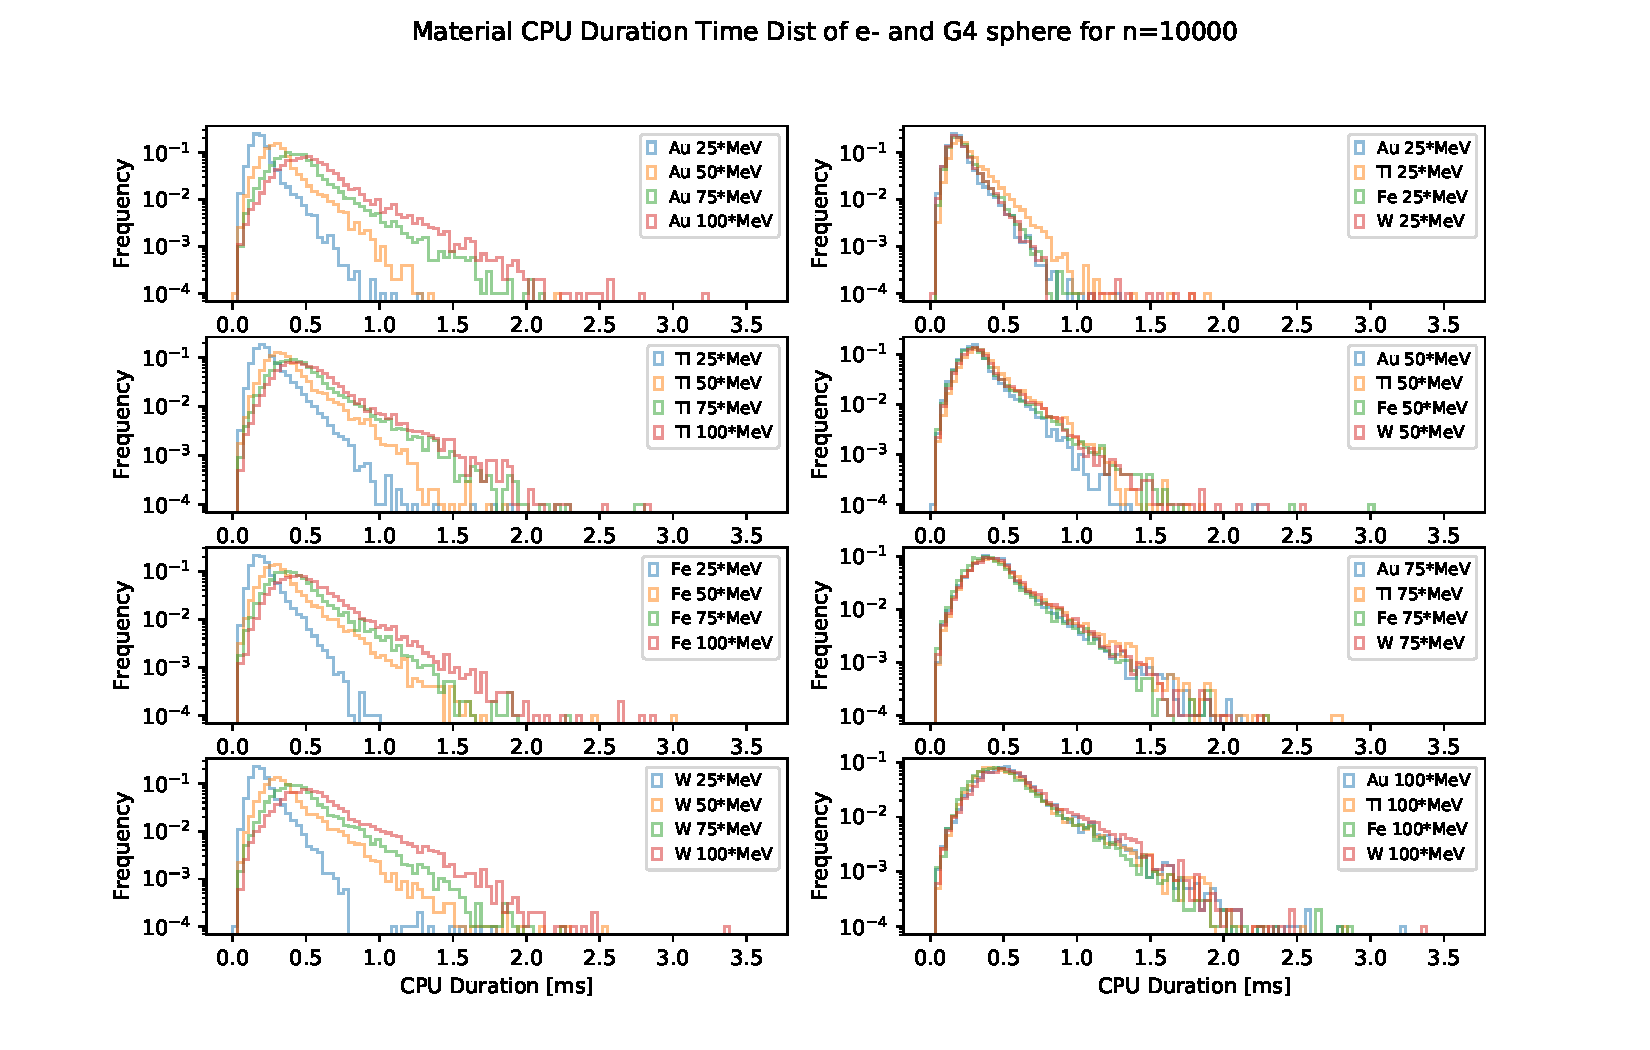
\includegraphics[scale=0.6]{Images//Materials//Varied_by_radius_and_secondaries.pdf}
\caption[width=\columnwidth]{Histograms showing the CPU duration distributions of varying materials and particle energies in BDSIM on a Geant4 sphere. The left 4 histograms show the distributions show the varying of energy on each material. The right 4 histograms show the varying of material at a set energy. Each plot is normalised by the initial 10,000 electrons in each event.}
\label{var}
\end{figure}

\noindent It can be seen that in Figure \ref{var}, the scaling of radius relative to stopping distances, generates histograms which act extremely similar at the same particle energies irrespective of the material it propagates through. This is very interesting as it means that for any further analysis, material can be ruled out as a variable and only energy needs to be varied.

\begin{figure}[h!]
\centering
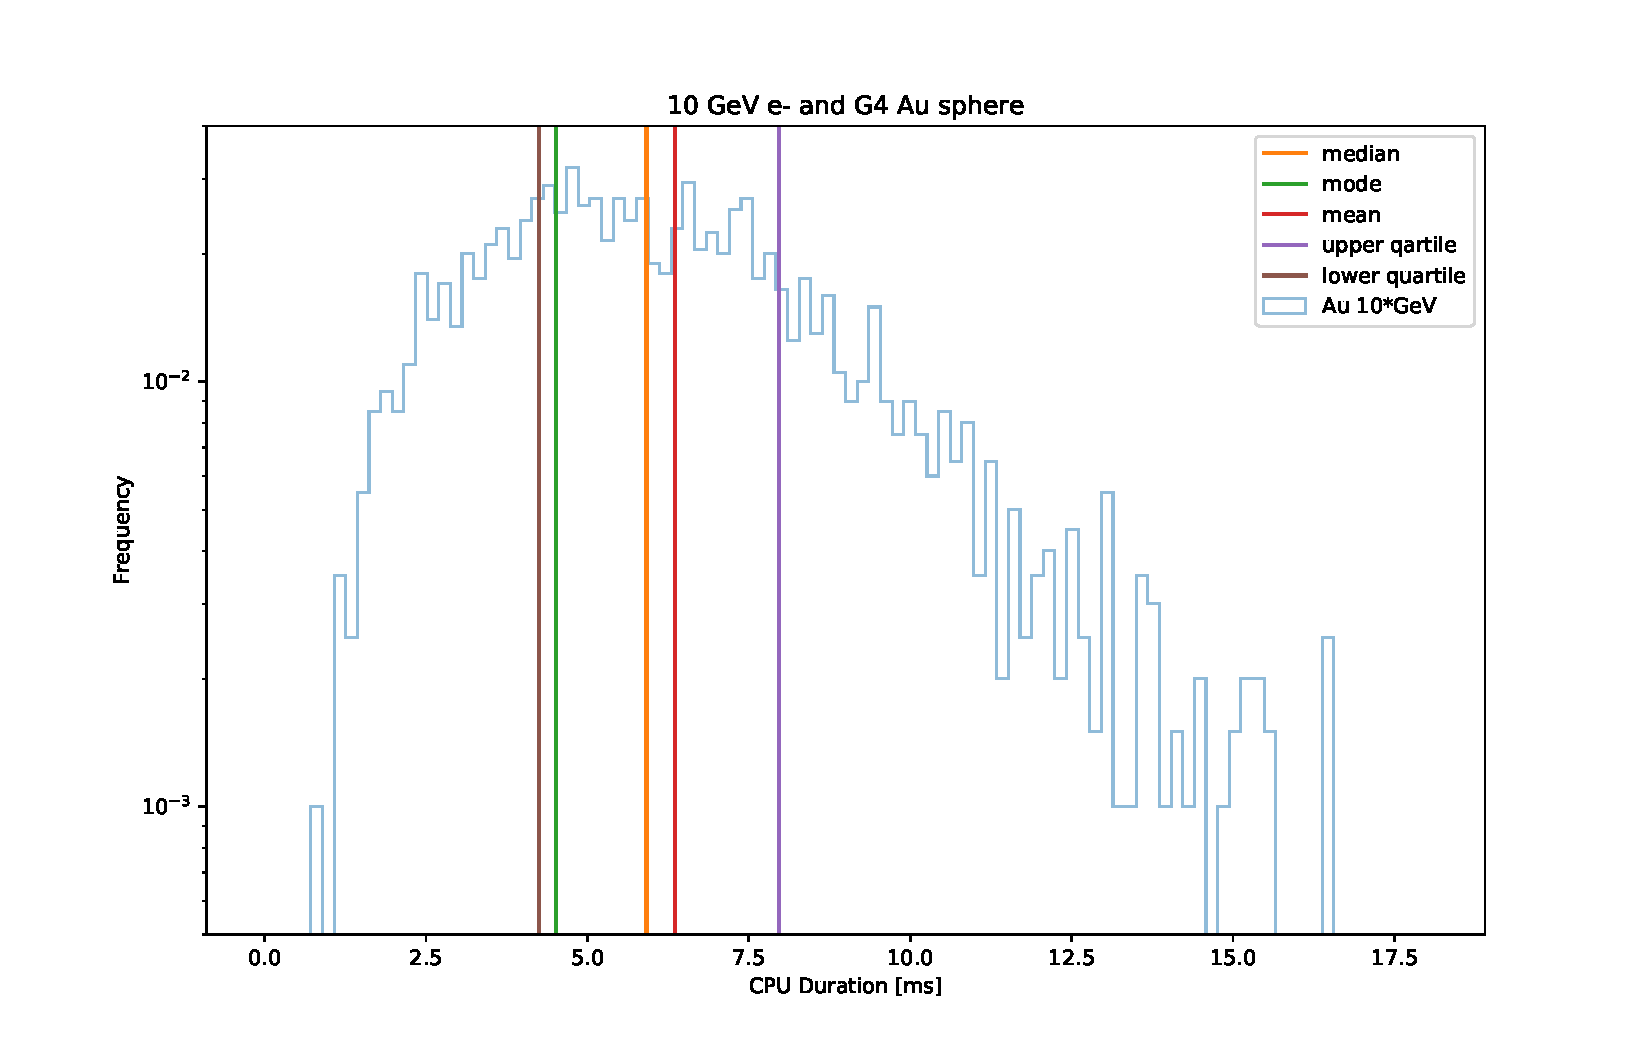
\includegraphics[scale=0.4]{Images//Materials//Time_ex_dists.pdf}
\caption[width=\columnwidth]{Meshing Development for Tubs (Solid \& Mesh View)}
\label{tubspic}
\end{figure}

\newpage
\subsection{Titanium Sphere Interactions \& Spherical Beam Distribution}
rmin = 0.01mm\\
rmax = 10mm\\
beam dist = sphere\\
10 GeV electrons\\
N decided by reduction\\

\begin{figure}[h!]
\centering
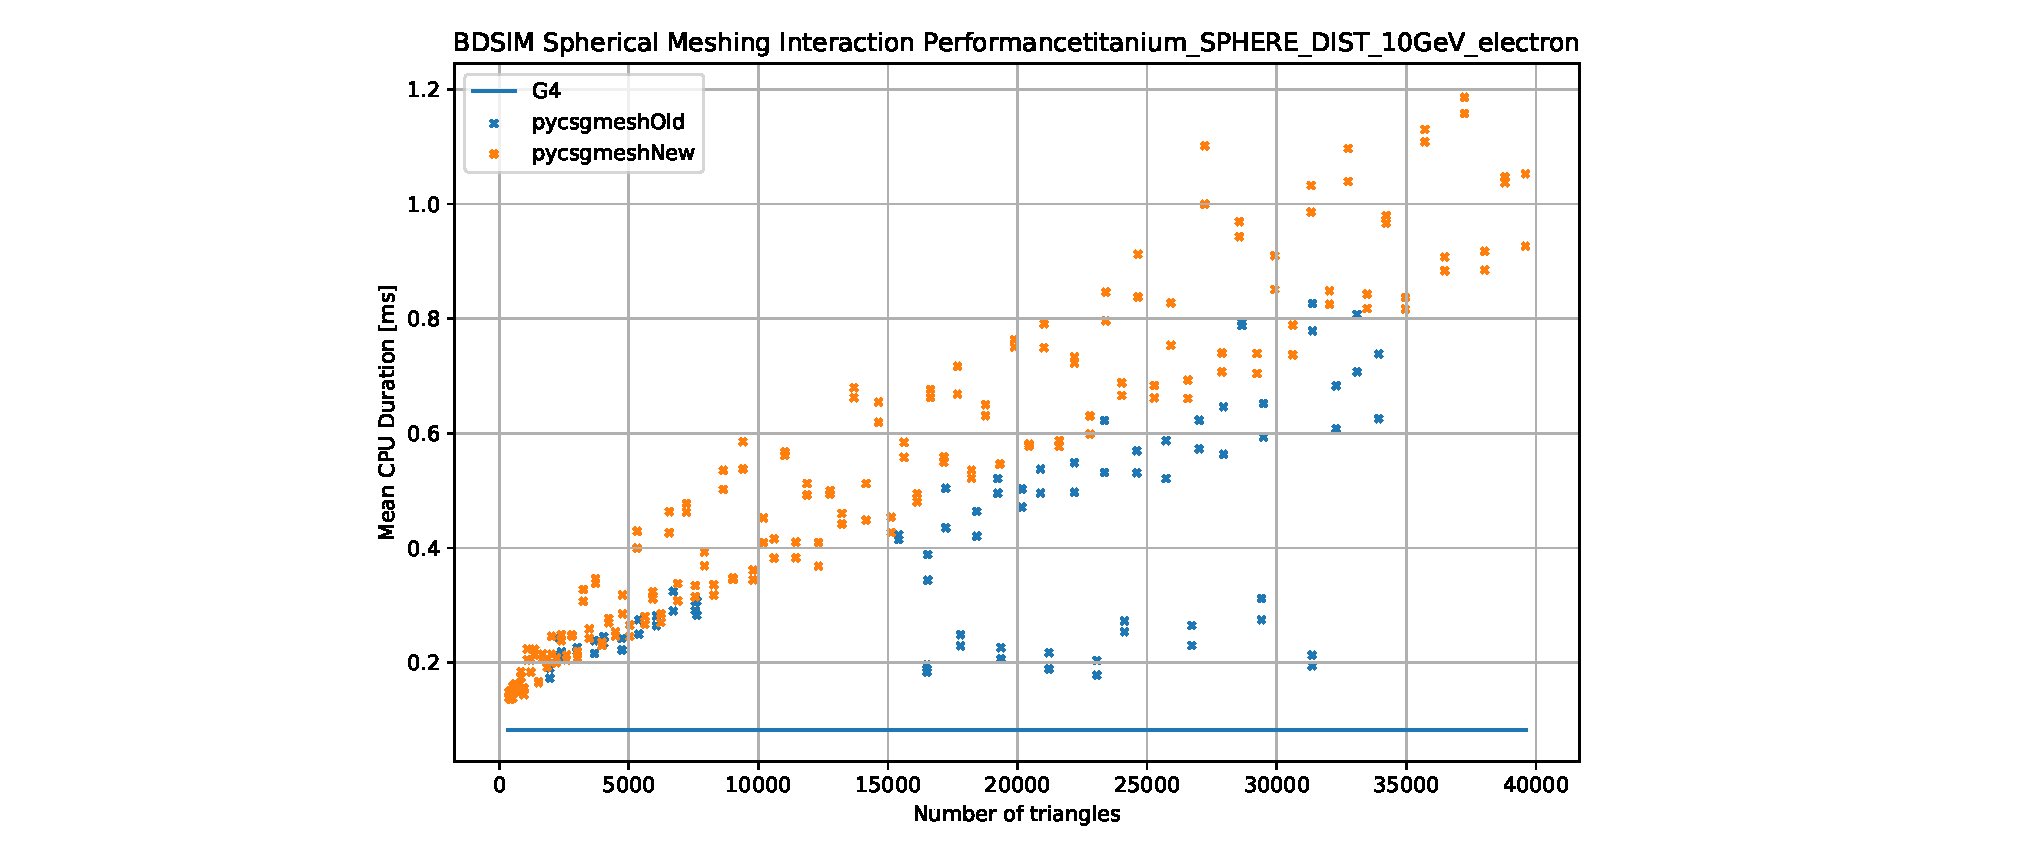
\includegraphics[scale=0.5]{Images//BDSIM//numoftris_tit_10G_e_nostd.pdf}
\caption[width=\columnwidth]{Meshing Development for Tubs (Solid \& Mesh View)}
\label{tubspic}
\end{figure}

\subsection{Interaction with CAD Magnet}
As a final goal to round off the project a compound boolean meshed solid of a real world magnet is analysed in the same way in which the meshed sphere was in the previous section. The CAD magnet is constructed out of basic primitive solids such that it can be compared between the old and new meshing methods.

\begin{figure}[h!]
\centering
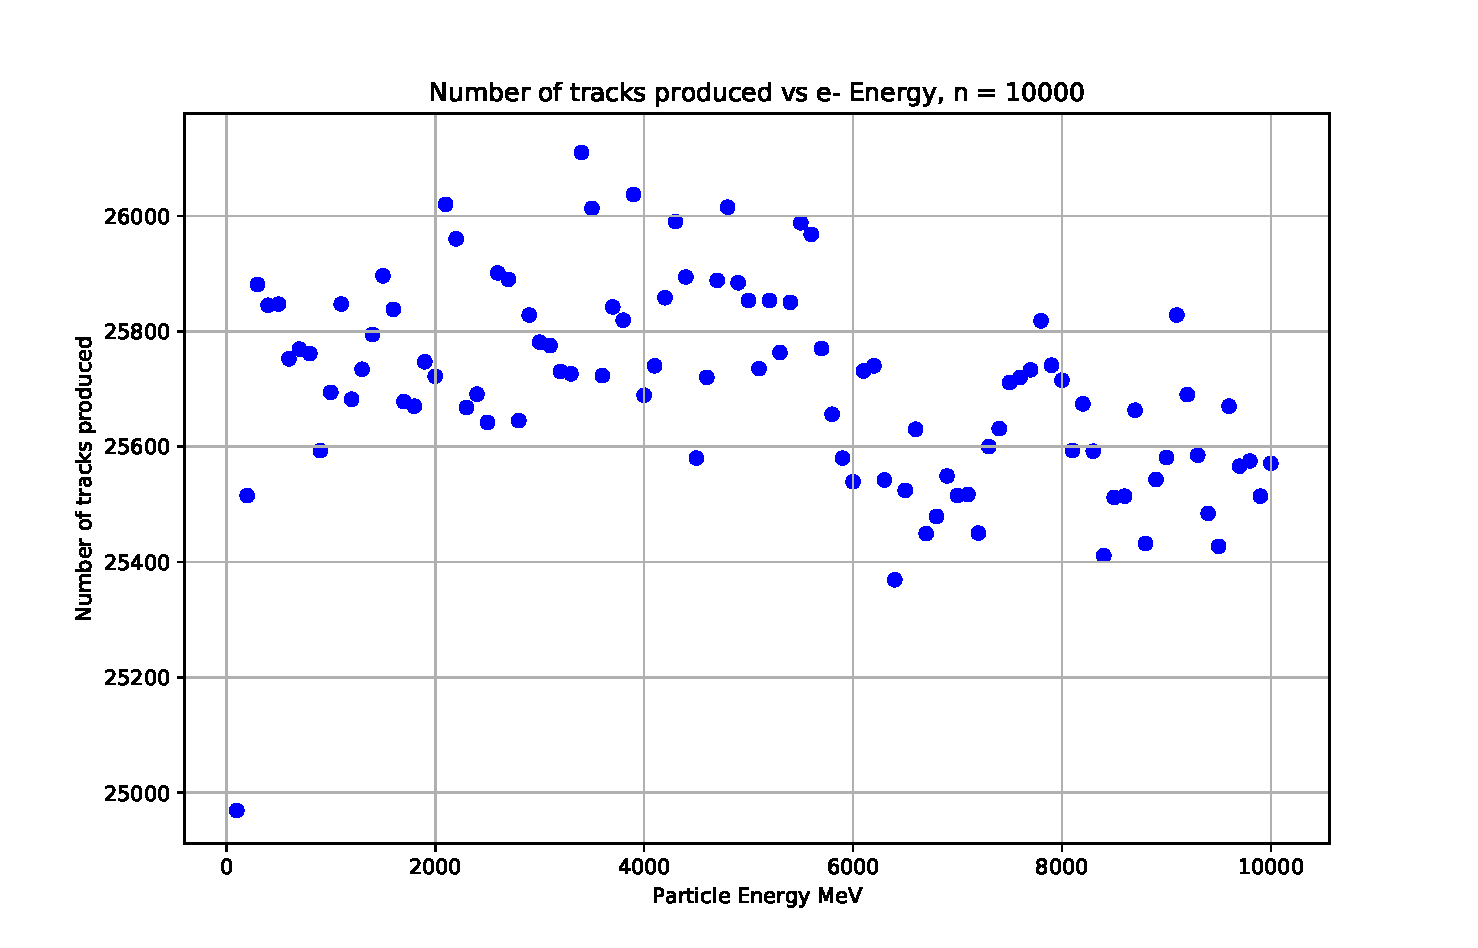
\includegraphics[scale=0.7]{Images//CAD_Mag//Secondaries_count.pdf}
\caption[width=\columnwidth]{BDSIM screenshot of 200 1.3 Gev protons interacting with a Iron sphere, generated with the new meshing using a stack \& slice of 10 \& 10. (Shown in mesh view)}
\label{sphbd}
\end{figure}

\newpage
\section{Conclusion \& Summary}
\label{conc}

\subsection{Improvements}
meshing is quicker\\
BDSIM interactions are quicker but still slower than G4 solid (as expected)
improved coverage unit test speeds\\
meshing is neater and more uniform in structure\\
higher meshing density = closer to true solid as expected with bdsim interactions\\
quote graphs and sections\\

\subsection{Applications}
BDSIM and Pyg4ometry are both very powerful software packages that can be used to to aid not only the scientific research community of particle physicist, but also help everyday people by improving medical treatment. Thanks to the software being open source and its wide range of file compatibilities it can be used to simulate a growing number of projects. This report demonstrates this by CAD magnet modelling.

% ------------------------------------------------------------------------------------------------------------------------------

\newpage
\begin{thebibliography}{1}

	\bibitem{cern}
	CERN Homepage\\
	\url{https://home.cern/}
	
	\bibitem{jai}
	JAI Homepage\\
	\url{https://www.adams-institute.ac.uk/}

	\bibitem{pyg4om}
	Stewart Boogert et al.\\
	PYG4OMETRY : A TOOL TO CREATE GEOMETRIES FOR GEANT4,\\
BDSIM, G4BEAMLINE AND FLUKA FOR PARTICLE LOSS AND\\
ENERGY DEPOSIT STUDIES\\
	\url{http://accelconf.web.cern.ch/AccelConf/ipac2019/papers/wepts054.pdf}

	
	\bibitem{bitb}
	Pyg4ometry BitBucket\\
	\url{https://bitbucket.org/jairhul/Pyg4ometry/src/}
	
	\bibitem{}
		BDSIM Manual\\
		\url{http://www.pp.rhul.ac.uk/bdsim/manual/}
	\bibitem{}
		BDSIM Paper\\
		\url{https://doi.org/10.1016/j.cpc.2020.107200}
		
	\bibitem{st}
		Sourcetree\\
		\url{https://www.sourcetreeapp.com/}
		
	\bibitem{}
	Geant4 Solids\\
	\url{http://geant4-userdoc.web.cern.ch/geant4-userdoc/UsersGuides/ForApplicationDeveloper/html/Detector/Geometry/geomSolids.html}
	
	\bibitem{mater}
	Geant4 Materials\\
	\url{http://geant4-userdoc.web.cern.ch/geant4-userdoc/UsersGuides/ForApplicationDeveloper/html/Appendix/materialNames.html}
	
	\bibitem{meh}
	M. Pinto, P. Gon\c{c}alves\\
	GUIMesh: A tool to import STEP geometries into Geant4 via GDML\\
	\url{https://doi.org/10.1016/j.cpc.2019.01.024}
		
	\bibitem{pdg}
	M. Tanabashi et al\\
	43. Monte Carlo Particle Numbering Scheme\\
	\url{http://pdg.lbl.gov/2019/reviews/rpp2019-rev-monte-carlo-numbering.pdf}
	
	\bibitem{stpdat}
	U.S. DEPARTMENT OF COMMERCE\\
	Stopping Powers and Ranges of
	Electrons and Positrons\\
	\url{https://www.govinfo.gov/content/pkg/GOVPUB-C13-139be796c7e56cb34375ad52db8ec5e7/pdf/GOVPUB-C13-139be796c7e56cb34375ad52db8ec5e7.pdf}
	


\end{thebibliography}

% ------------------------------------------------------------------------------------------------------------------------------

\newpage
\appendix

\section{Appendix (Python scripts)}
\subsection{Sphere BDSIM Vary Mesh Test}
\label{ap1}
\lstinputlisting[language=Python]{Scripts//Run_New_Meshes.py}

%\newpage
%\subsection{Discovery method contribution pie chart (Figure \ref{pie})}\label{ap2}
%\lstinputlisting[language=Python]{Python//pi.py}

\newpage
\twocolumn[\section{All Meshed Solids and Polygon Count Plots}
\label{app1}
The following Figures are the meshing and polygon data for each primitive solid constructed in Pyg4ometry \ref{pyg}. The first Figure for each solid is a screenshot of the old meshing and new meshing visualized in VTK. They show the before and after of each primitive solid in both "solid view" and "mesh view". The second Figures Show the number of polygons and triangles produced by the solid as you increase the slice across a range of 10-100 (if there is a stack it is kept at a constant 10). The polygon data plots are generate using python 2.7. The naming convention is the one used by Geant4 \ref{g4}.\\]
\begingroup
\subsubsection{Cons}
\begin{figure}[h!]
\centering
\begin{minipage}{.2\textwidth}
  \centering
  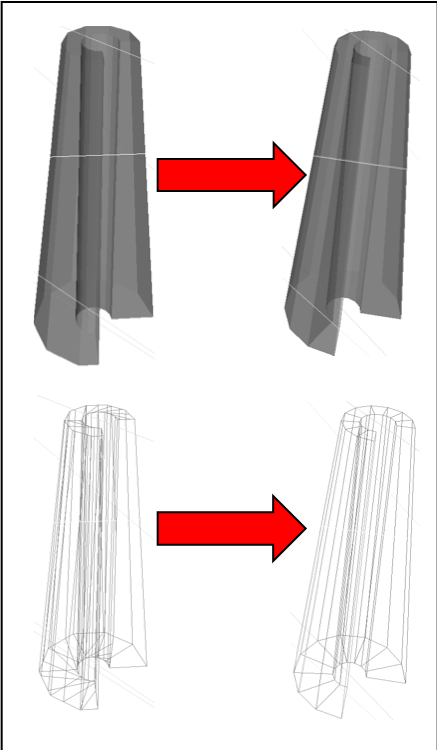
\includegraphics[height=1\linewidth]{Images//Meshes//cons.png}
  \captionof{figure}{}
  \label{cons}
\end{minipage}%
\begin{minipage}{.3\textwidth}
  \centering
  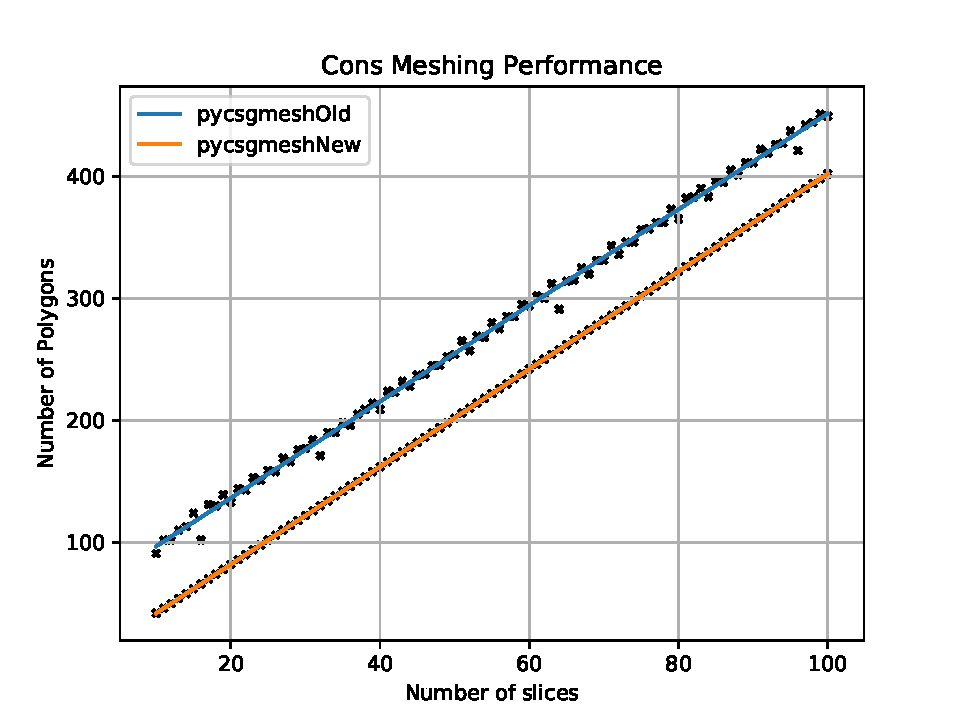
\includegraphics[scale=0.35]{Images//Quad_fits//Cons_quad.pdf}
  \captionof{figure}{ }
  \label{fig:test2}
\end{minipage}%
\end{figure}

\subsubsection{CutTubs}

\begin{figure}[h!]
\centering
\begin{minipage}{.2\textwidth}
  \centering
  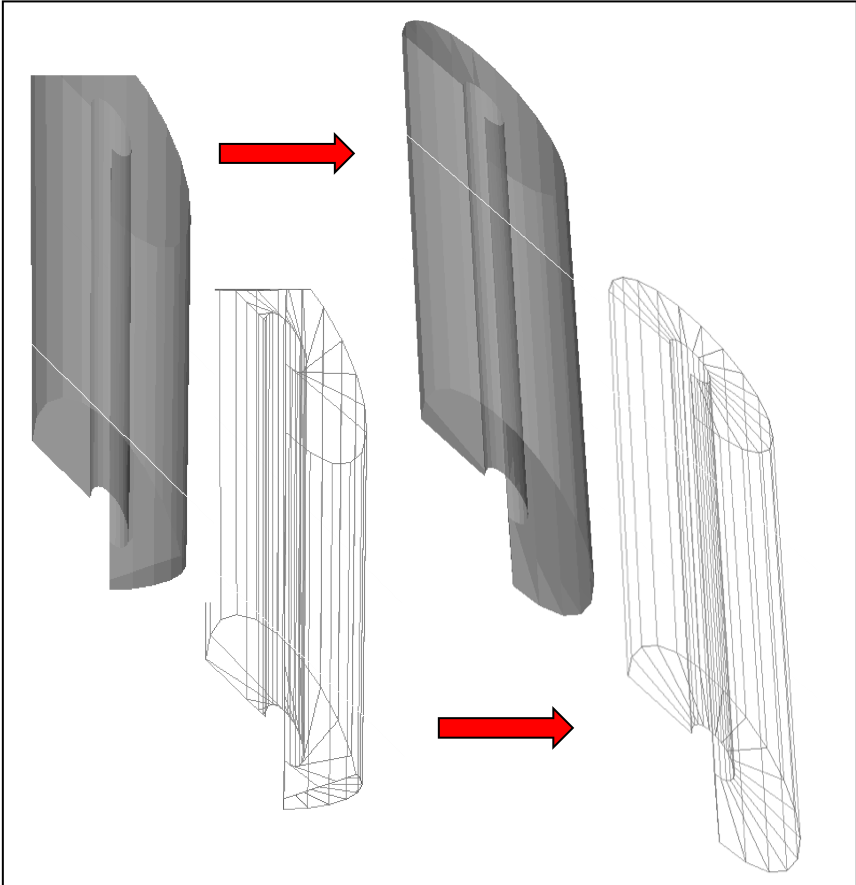
\includegraphics[height=1\linewidth]{Images//Meshes//CutTubs.png}
  \captionof{figure}{ }
  \label{ctub}
\end{minipage}%
\begin{minipage}{.3\textwidth}
  \centering
  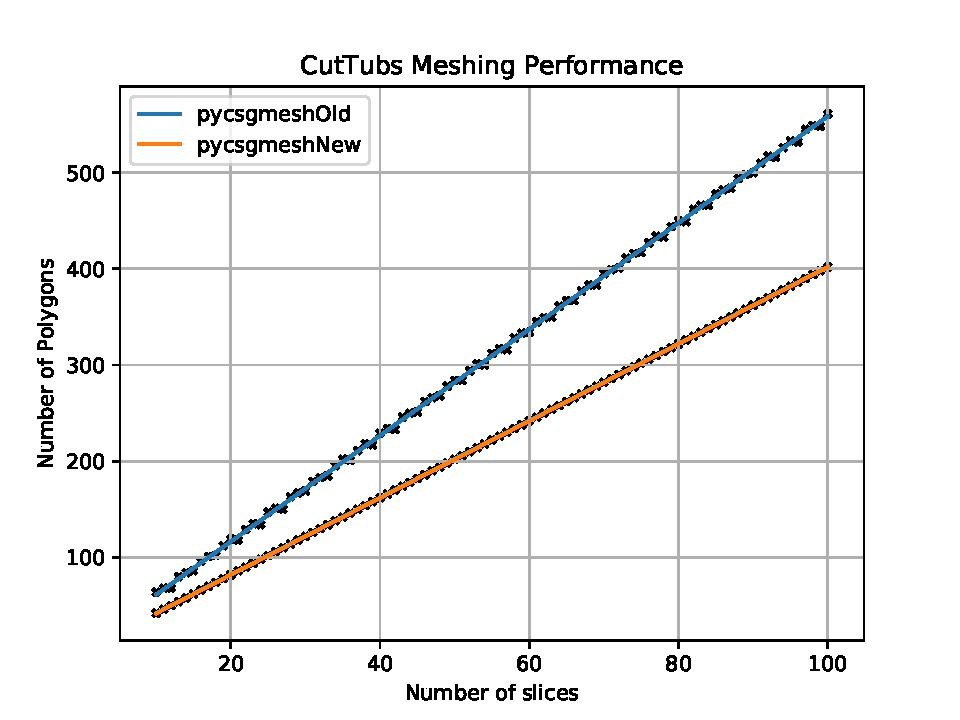
\includegraphics[scale=0.35]{Images//Quad_fits//CutTubs_quad.pdf}
  \captionof{figure}{ }
  \label{}
\end{minipage}%
\end{figure}

\subsubsection{Ellipsoid}

\begin{figure}[h!]
\centering
\begin{minipage}{.2\textwidth}
  \centering
  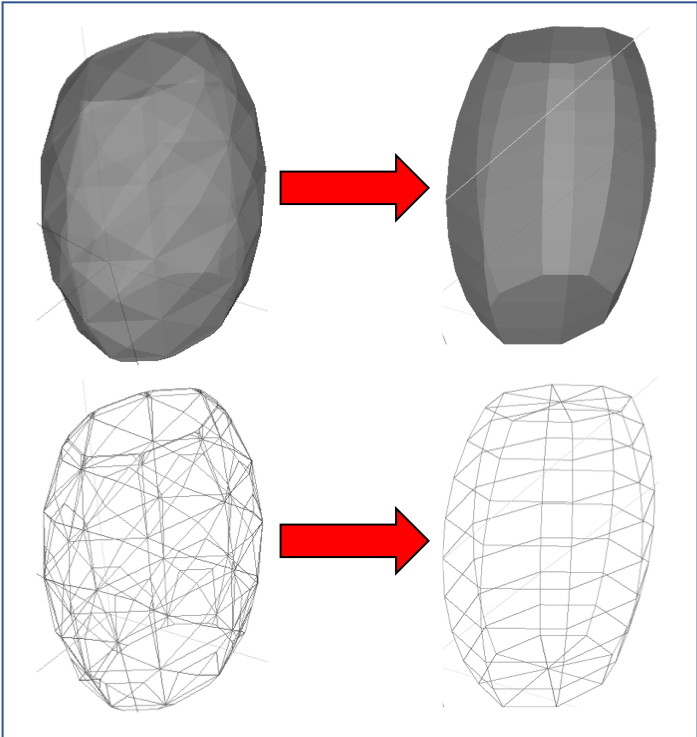
\includegraphics[height=1\linewidth]{Images//Meshes//ellipsoid.png}
  \captionof{figure}{ }
  \label{fig:test1}
\end{minipage}%
\begin{minipage}{.3\textwidth}
  \centering
  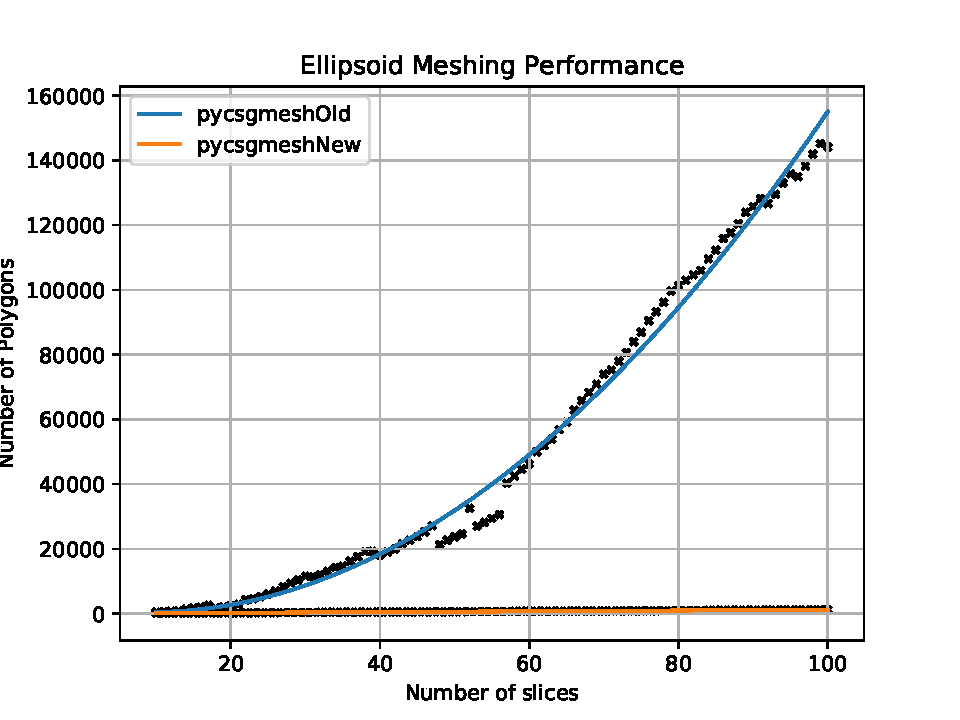
\includegraphics[scale=0.35]{Images//Quad_fits//Ellipsoid_quad.pdf}
  \captionof{figure}{ }
  \label{fig:test2}
\end{minipage}%
\end{figure}

\newpage
\subsubsection{EllipticalCone}

\begin{figure}[h!]
\centering
\begin{minipage}{.2\textwidth}
  \centering
  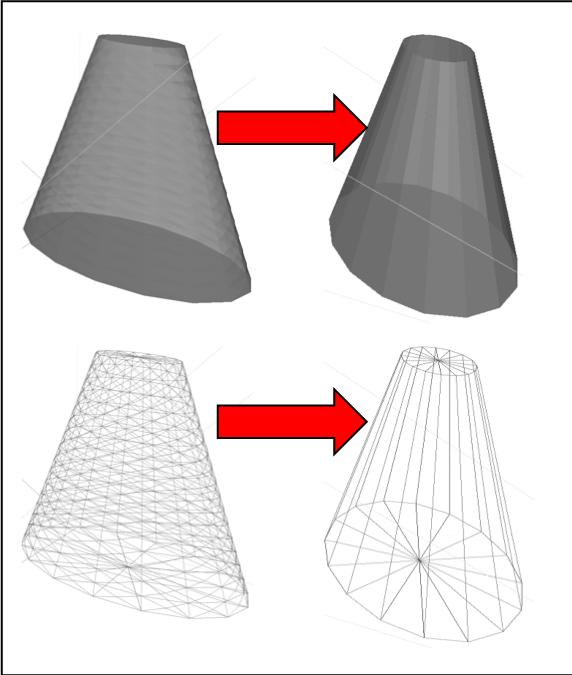
\includegraphics[height=1\linewidth]{Images//Meshes//ellipticalcone.png}
  \captionof{figure}{ }
  \label{fig:test1}
\end{minipage}%
\begin{minipage}{.3\textwidth}
  \centering
  \includegraphics[scale=0.35]{Images//Quad_fits//Ellipticalcone_quad.pdf}
  \captionof{figure}{ }
  \label{fig:test2}
\end{minipage}%
\end{figure}

\subsubsection{EllipticalTube}

\begin{figure}[h!]
\centering
\begin{minipage}{.2\textwidth}
  \centering
  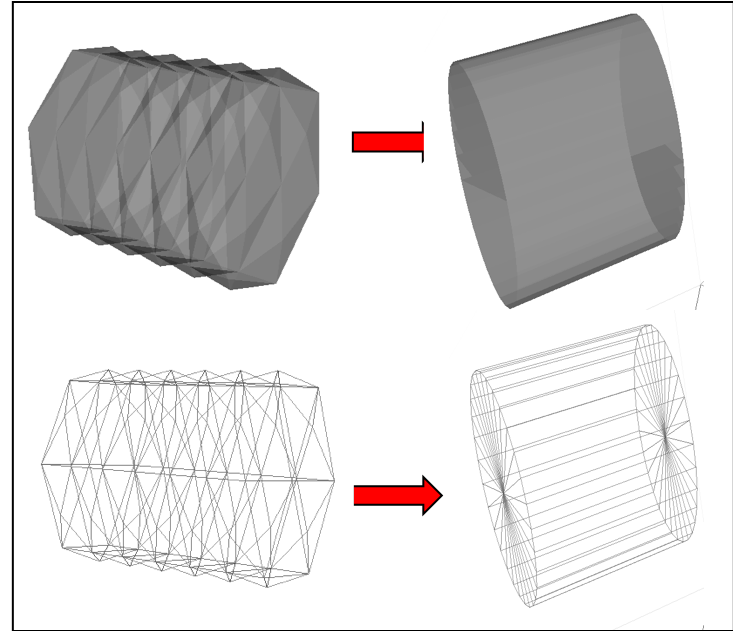
\includegraphics[height=0.8\linewidth]{Images//Meshes//ellipticaltube.png}
  \captionof{figure}{ }
  \label{fig:test1}
\end{minipage}%
\begin{minipage}{.3\textwidth}
  \centering
  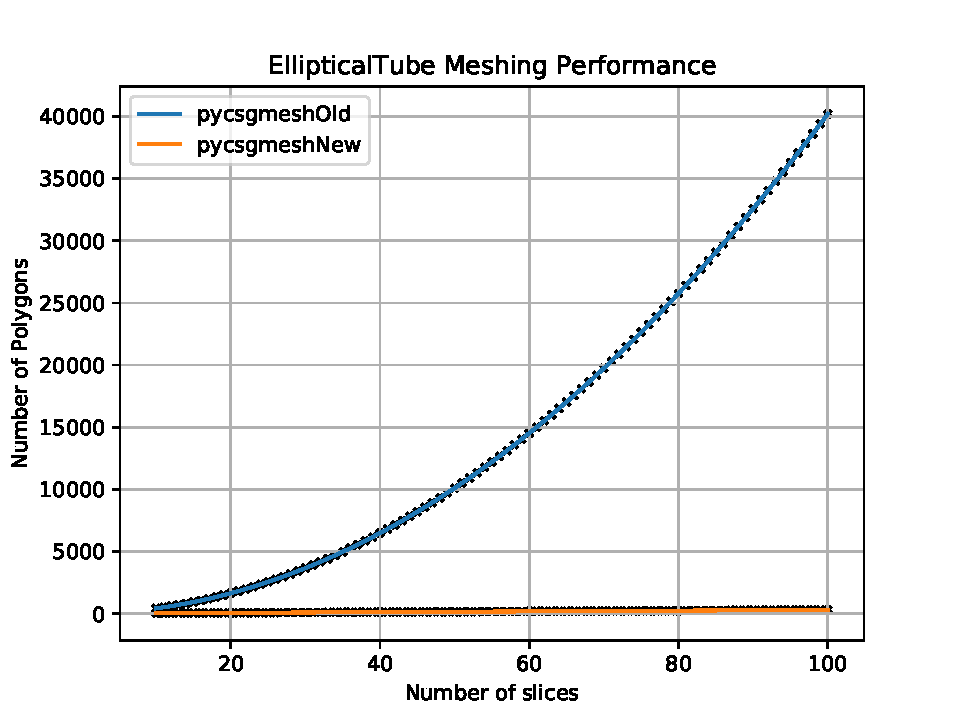
\includegraphics[scale=0.35]{Images//Quad_fits//EllipticalTube_quad.pdf}
  \captionof{figure}{ }
  \label{fig:test2}
\end{minipage}%
\end{figure}

\subsubsection{Hyperboloid}

\begin{figure}[h!]
\centering
\begin{minipage}{.2\textwidth}
  \centering
  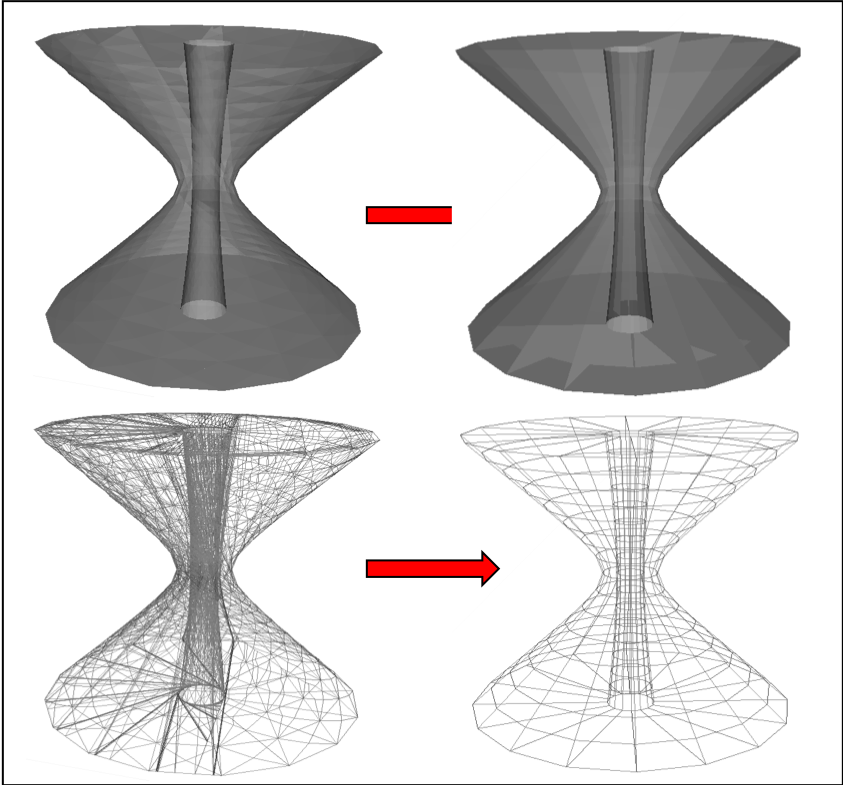
\includegraphics[height=0.9\linewidth]{Images//Meshes//hyperboloid.png}
  \captionof{figure}{ }
  \label{fig:test1}
\end{minipage}%
\begin{minipage}{.3\textwidth}
  \centering
  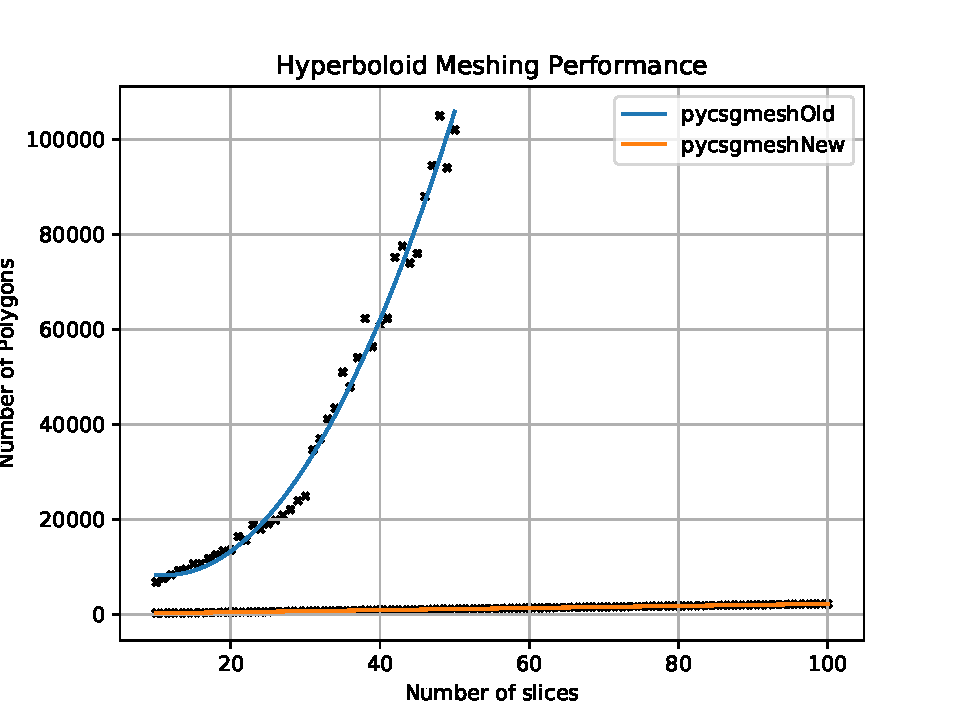
\includegraphics[scale=0.35]{Images//Quad_fits//Hyperboloid_quad.pdf}
  \captionof{figure}{ }
  \label{fig:test2}
\end{minipage}%
\end{figure}

\newpage
\subsubsection{Orb}

\begin{figure}[h!]
\centering
\begin{minipage}{.2\textwidth}
  \centering
  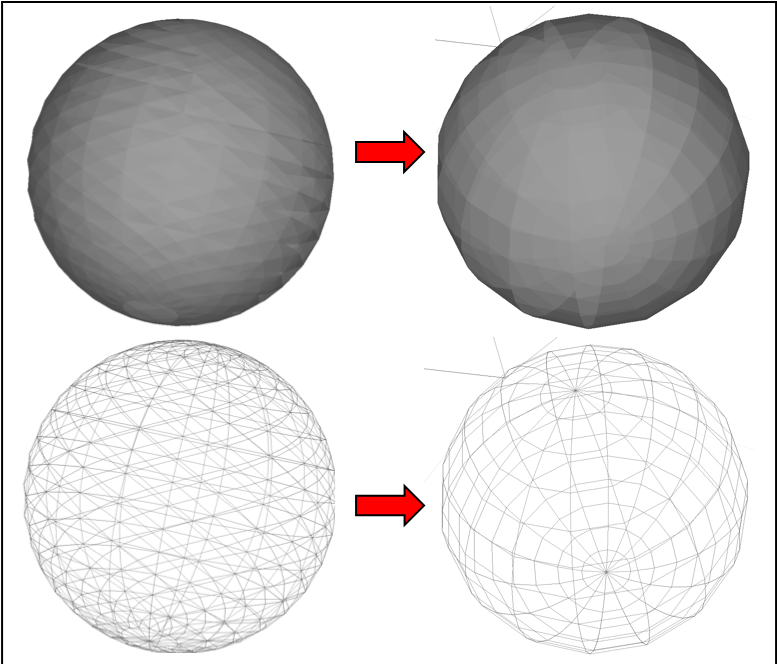
\includegraphics[height=0.8\linewidth]{Images//Meshes//orb.png}
  \captionof{figure}{ }
  \label{Sphere}
\end{minipage}%
\begin{minipage}{.3\textwidth}
  \centering
  \includegraphics[scale=0.35]{Images//Quad_fits//orb_quad.pdf}
  \captionof{figure}{ }
  \label{fig:test2}
\end{minipage}%
\end{figure}

\subsubsection{Paraboloid}

\begin{figure}[h!]
\centering
\begin{minipage}{.2\textwidth}
  \centering
  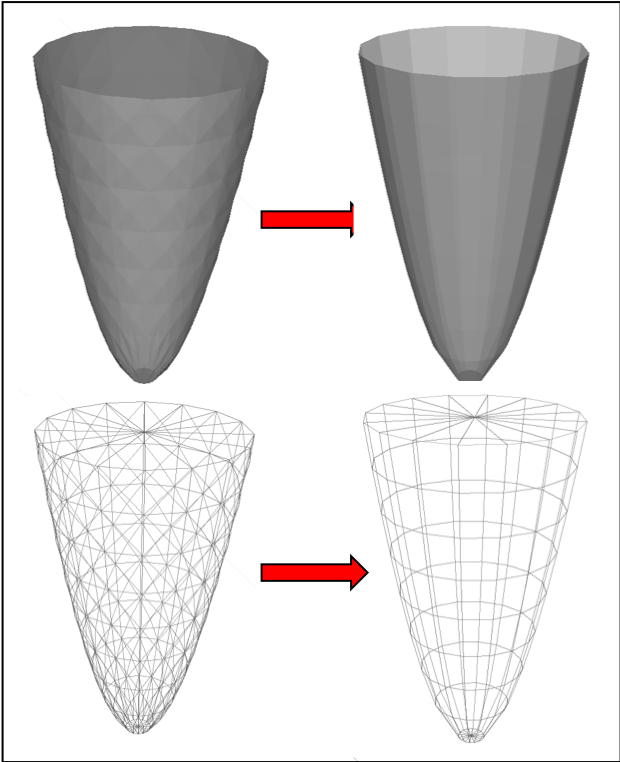
\includegraphics[height=1\linewidth]{Images//Meshes//paraboloid.png}
  \captionof{figure}{ }
  \label{para}
\end{minipage}%
\begin{minipage}{.3\textwidth}
  \centering
  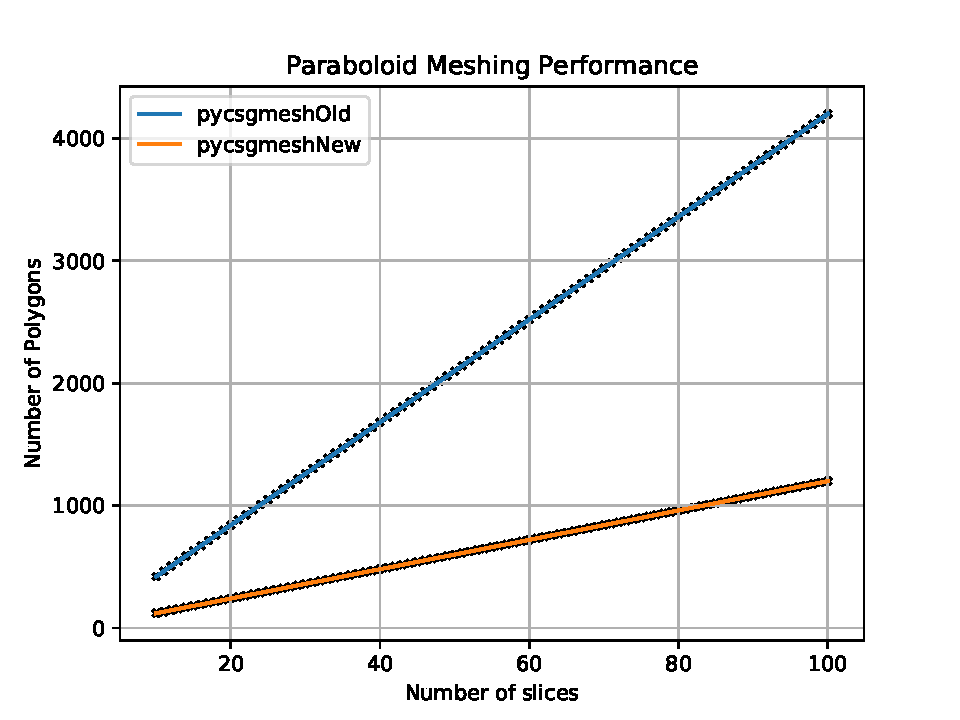
\includegraphics[scale=0.35]{Images//Quad_fits//Paraboloid_quad.pdf}
  \captionof{figure}{ }
  \label{fig:test2}
\end{minipage}%
\end{figure}

\subsubsection{Polycone}
\begin{figure}[h!]
\centering
\begin{minipage}{.2\textwidth}
  \centering
  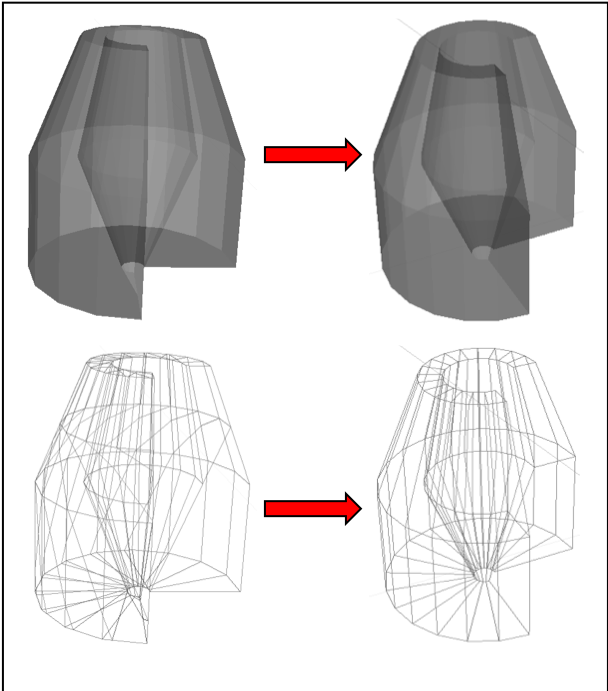
\includegraphics[height=1\linewidth]{Images//Meshes//polycone.png}
  \captionof{figure}{ }
  \label{fig:test1}
\end{minipage}%
\begin{minipage}{.3\textwidth}
  \centering
  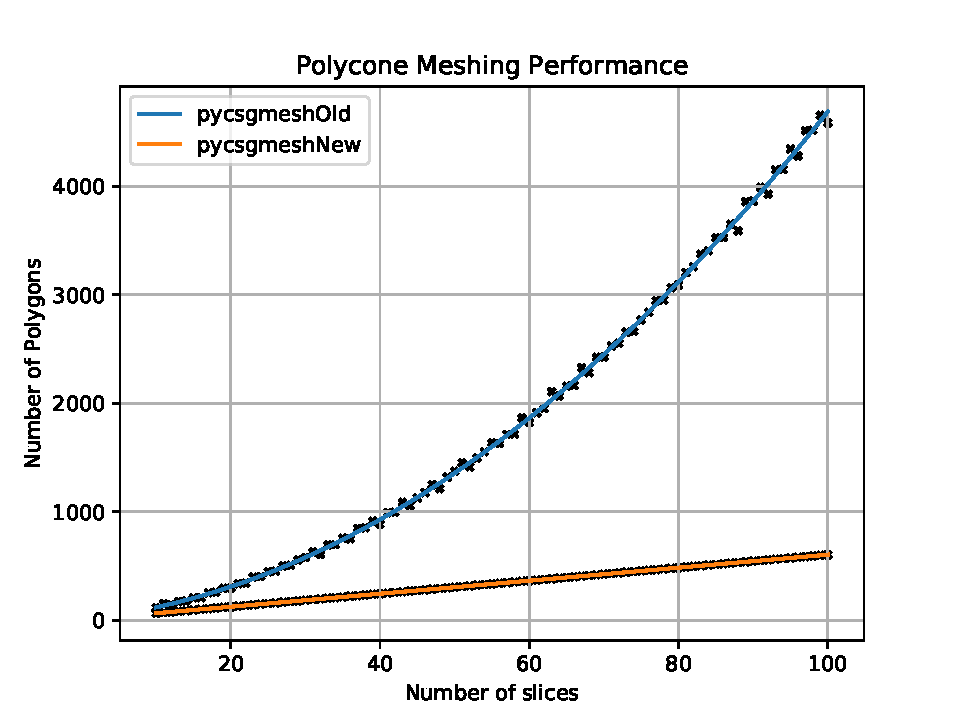
\includegraphics[scale=0.35]{Images//Quad_fits//Polycone_quad.pdf}
  \captionof{figure}{ }
  \label{fig:test2}
\end{minipage}%
\end{figure}

\newpage
\subsubsection{Sphere}
\begin{figure}[h!]
\centering
\begin{minipage}{.2\textwidth}
  \centering
  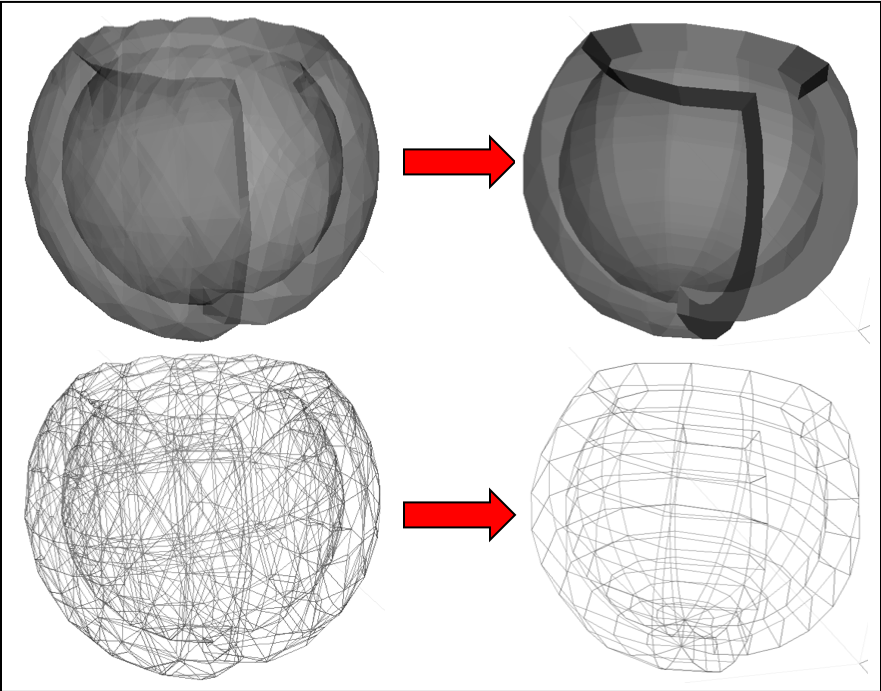
\includegraphics[height=0.75\linewidth]{Images//Meshes//sphere.png}
  \captionof{figure}{ }
  \label{fig:test1}
\end{minipage}%
\begin{minipage}{.3\textwidth}
  \centering
  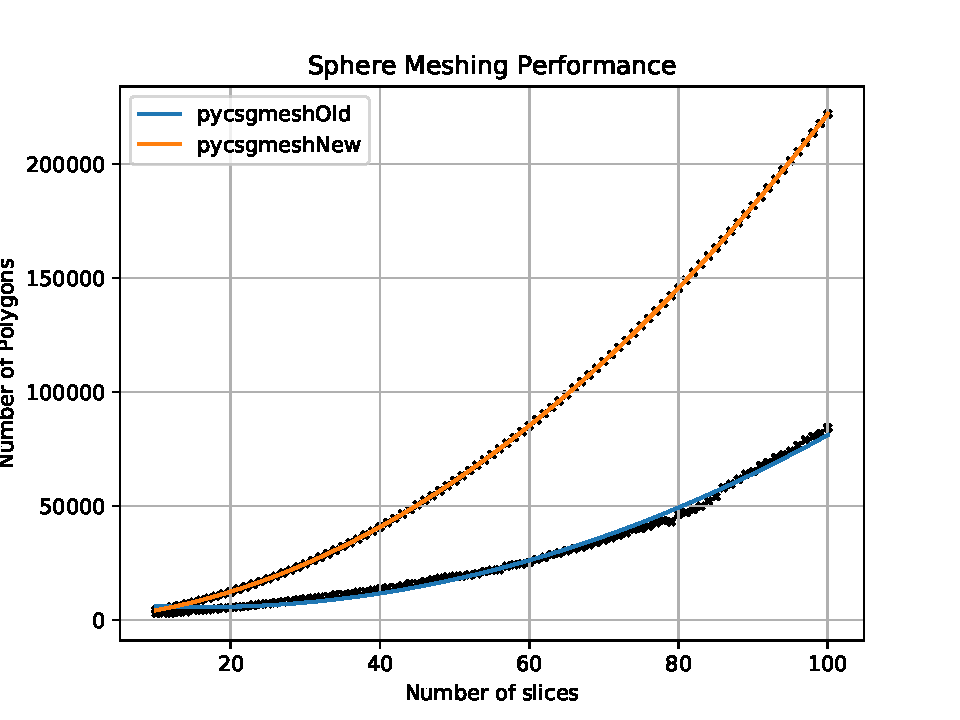
\includegraphics[scale=0.35]{Images//Quad_fits//Sphere_quad.pdf}
  \captionof{figure}{ }
  \label{fig:test2}
\end{minipage}%
\end{figure}

\subsubsection{Torus}

\begin{figure}[h!]
\centering
\begin{minipage}{.2\textwidth}
  \centering
  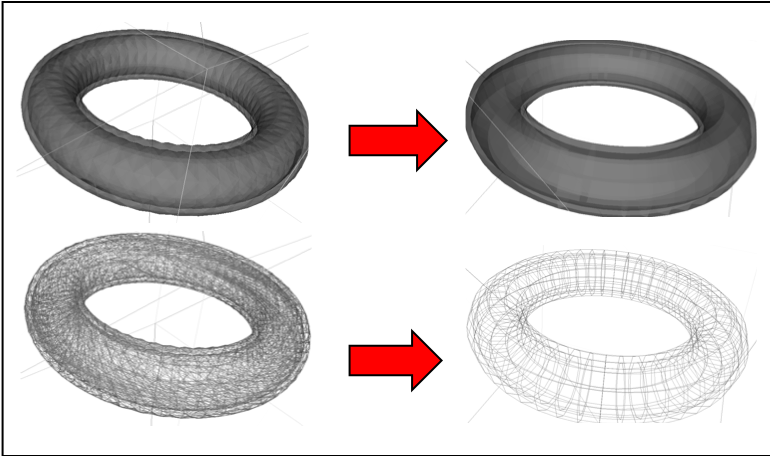
\includegraphics[height=0.5\linewidth]{Images//Meshes//torus.png}
  \captionof{figure}{ }
  \label{fig:test1}
\end{minipage}%
\begin{minipage}{.3\textwidth}
  \centering
  \includegraphics[scale=0.35]{Images//Quad_fits//Torus_quad.pdf}
  \captionof{figure}{ }
  \label{fig:test2}
\end{minipage}%
\end{figure}

\subsubsection{Tubs}

\begin{figure}[h!]
\centering
\begin{minipage}{.2\textwidth}
  \centering
  \includegraphics[height=0.7\linewidth]{Images//Meshes//tubs.png}
  \captionof{figure}{ }
  \label{fig:test1}
\end{minipage}%
\begin{minipage}{.3\textwidth}
  \centering
  \includegraphics[scale=0.35]{Images//Quad_fits//Tubs_quad.pdf}
  \captionof{figure}{ }
  \label{fig:test2}
\end{minipage}%
\end{figure}

\endgroup
\onecolumn
\section{Quadratic Parameters for polygon count plots}
\label{appp1}
The quadratic fit where its parameters are of the form:
\begin{equation}
ax^2 + bx + c = 0
\end{equation}

\small
% Table generated by Excel2LaTeX from sheet 'Sheet1'
\begin{table}[htbp]
  \small
  \centering
  \caption{A Table showing the parameters to the quadratic fits for the polygon count plot.}
    \begin{tabular}{lrrrrrr}
    Curved Primitive Solid & \multicolumn{1}{l}{Old a} & \multicolumn{1}{l}{Old b} & \multicolumn{1}{l}{Old c} & \multicolumn{1}{l}{New a} & \multicolumn{1}{l}{New b} & \multicolumn{1}{l}{New c} \\
    Cons  & -2.74E-04 & 3.97E+00 & 5.72E+01 & -3.83E-17 & 4.00E+00 & 2.00E+00 \\
    CutTubs & 2.19E-04 & 5.50E+00 & 6.30E+00 & -3.83E-17 & 4.00E+00 & 2.00E+00 \\
    Ellipsoid & 18.65090372 & -333.5688153 & 1919.792901 & 1.61E-17 & 1.20E+01 & 0.00E+00 \\
    EllipticalCone & 4.00E+00 & 2.00E+00 & 2.41E-12 & 4.03E-18 & 3.00E+00 & 0.00E+00 \\
    EllipticalTube & -1.94E-16 & 4.20E+01 & -5.72E-13 & 4.03E-18 & 3.00E+00 & 0.00E+00 \\
    Hyperboloid & 64.83177713 & -1452.629624 & 16378.18198 & 4.84E-17 & 2.20E+01 & -9.53E-14 \\
    Orb   & -6.45E-17 & 3.40E+01 & -1.91E-13 & -8.06E-18 & 1.00E+01 & -4.77E-14 \\
    Paraboloid & -1.94E-16 & 3.40E+01 & -1.91E-13 & 1.61E-17 & 1.20E+01 & 0.00E+00 \\
    Polycone & 0.39682347 & 7.13011557 & 7.42466252 & -4.03E-17 & 6.00E+00 & 4.00E+00 \\
    Sphere & 10.82154926 & -356.6329124 & 8557.249195 & 2.00E+01 & 2.20E+02 & 1.98E-11 \\
    Torus & 7.01776508 & 304.8746037 & 4899.196225 & -1.61E-17 & 2.00E+01 & -9.53E-14 \\
    Tubs  & 0.27241769 & 4.58191175 & 8.33675211 & -3.83E-17 & 4.00E+00 & 2.00E+00 \\
    \end{tabular}%
  \label{tab1}%
\end{table}


\end{document}

